\documentclass[a4paper,12pt]{skthesis}
%\usepackage{lgrind}  % not needed with xelatex
%\usepackage{cmap}    % not needed with xelatex
%\usepackage[T2A]{fontenc}


% \newcommand{\gfcb}[1]{%
%     \fcolorbox{white}{gray!10!}{\quad\strut #1\quad}
%     } % gfcb := gray fcolorbox
% \newcommand{\cop}[1]{%
%     \texttt{\detokenize{#1}} 
%     } % cop := code output
\usepackage{csquotes} 
\usepackage{hyperref}
\usepackage{nameref}

\setcounter{secnumdepth}{2}

\begin{document}
% Everything with --rus inside is supposed to be written in russian

\title{Revisiting the L\'evy Foraging Hypothesis in 2D with Reproducible Simulation}
\titlerus{Повторное исследование гипотезы Леви о фуражировке в 2D с воспроизводимым моделированием}

\author{Anita Toleutaeva}
\authorrus{Анита Толеутаева}

\department{Advanced Computational Science}
\departmentrus{Современные вычислительные методы}

%\degree{Master of Energy Systems}
%\degreerus{Мастер энергетических систем}

\degreemonth{June}
\degreeyear{2026}
\thesisdate{}
\degreemonthrus{Июнь}
\thesisdaterus{}

\supervisorname{Vladimir Palyulin}
\supervisortitle{Associate professor}
\supervisordegree{PhD}

\supervisornamerus{Владимир Палюлин}
\supervisortitlerus{доцент}
\supervisordegreerus{к.ф.-м.н.}


% If you have cosupervisor, uncomment and fill these lines with name, title and degree of your cosupervisor
% Name and title fields are mandatory!

% If you have two co-advisors uncomment the lines below
% \cocosupervisorname{Name2 Surname2}
% \cocosupervisortitle{Senior research scientist}
% \cocosupervisordegree{PhD}

% \cocosupervisornamerus{Имя Фамилия}
% \cocosupervisortitlerus{научный сотрудник}
% \cocosupervisordegreerus{д.ф.-м.н.}


\maketitle
\rusmaketitle

\setcounter{savepage}{\thepage}

\keywords{L\'evy flights, random search, optimal foraging, L\'evy foraging hypothesis, mean first-passage time, Monte Carlo simulation, heavy-tailed distributions.}
\begin{abstractpage}

Random search arises whenever an agent must locate sparse targets with little or no sensory guidance---from animal foraging to exploration, rescue, and resource prospecting---and a central open question is which movement statistics are optimal under controlled assumptions. The L\'evy foraging hypothesis proposes that scale-free motion with power-law relocation lengths can be near-optimal in two-dimensional search, yet published conclusions remain highly model-dependent because implementation details (e.g., destructive vs.\ nondestructive targets, whether relocations are interrupted by detections, and how revisits are handled) vary across studies.

In this work we develop a transparent, reproducible 2D simulation framework for step-by-step random search on an infinite plane with Poisson-distributed targets, making modeling choices explicit while avoiding ad hoc reset rules. Within a unified framework, we compare four post-detection strategies---no-interrupt, teleport, and Viswanathan restart in both destructive and non-destructive modes---sweeping the L\'evy exponent $\mu \in [1, 3]$ (equivalently, tail exponent $\alpha = \mu - 1 \in [0, 2]$). Performance is measured primarily by the pooled unique-capture rate; mean first-passage time is analyzed for selected cases. Extensive Monte Carlo simulations across sparsity levels $\lambda/r_v \in [10, 2000]$, combined with sensitivity analyses of truncation parameters and convergence studies, yield an empirical regime map of the optimal exponent $\mu^*$. The results are consistent with $\mu^* \approx 2$ ($\alpha \approx 1$) in the sparsest tested regimes for all four strategies, show a shift toward ballistic motion ($\mu^* \to 1$) at high target density for three of four strategies, and document a trapping pathology in the non-destructive zero-jump-off implementation.

\end{abstractpage}

\setcounter{page}{\thesavepage}
\begin{abstractpagerus}
\selectlanguage{russian}
Случайный поиск возникает в задачах, где агенту нужно находить редкие цели при почти полном отсутствии информации о среде: от кормодобывания животных до разведки местности, поисково-спасательных работ и поиска ресурсов. Один из ключевых открытых вопросов — какие законы движения дают наилучшие результаты при фиксированных и чётко заданных предположениях. Гипотеза о «поиске Леви» утверждает, что безмасштабное движение со степенным распределением длин перемещений может быть близким к оптимальному в двумерном пространстве. Однако выводы разных работ плохо согласуются между собой, поскольку сильно зависят от того, как именно сформулирована и реализована модель: рассматриваются ли цели как исчерпаемые или возобновляемые, прерываются ли перемещения при обнаружении, и каким образом учитываются повторные посещения.

В данной работе разработан прозрачный и воспроизводимый двумерный программный комплекс для пошагового случайного поиска на бесконечной плоскости с пуассоновским распределением целей. Модельные решения задаются явно и исключаются произвольные правила «сброса». В рамках единой постановки сравниваются четыре стратегии пост-обнаружения: продолжение полёта, телепортация и перезапуск по Висванатану в разрушающем и неразрушающем режимах. Проводится перебор показателя Леви $\mu \in [1, 3]$ (эквивалентно, хвостовой показатель $\alpha = \mu - 1 \in [0, 2]$). Эффективность оценивается главным образом по объединённой частоте уникальных обнаружений; среднее расстояние до первого обнаружения анализируется для отдельных случаев. Масштабное моделирование методом Монте-Карло для уровней разреженности $\lambda/r_v \in [10, 2000]$, дополненное анализом чувствительности параметров усечения и исследованием сходимости, позволяет построить эмпирическую карту режимов оптимального показателя $\mu^*$. Результаты согласуются с оценкой $\mu^* \approx 2$ ($\alpha \approx 1$) при наиболее разреженных протестированных условиях, показывают смещение к баллистическому движению ($\mu^* \to 1$) при высокой плотности для трёх из четырёх стратегий и документируют патологию «захвата» в неразрушающем режиме с нулевым расстоянием сброса.

\end{abstractpagerus}

%%%%%%%%%%%%%%%%%%%%%%%%%%%%%%%%%%%%%%%%%%%%%%%%%%%%%%%%%%%%%%%%%%%%%%
% -*-latex-*-
 % Your title pages, abstract
\include{chapters/contents} % Probably you don't need to change it
\chapter{Introduction}
\label{ch:introduction}

\textbf{Foraging} is the process by which an organism searches for and exploits resources (typically food, but also mates, shelter, or other essential “targets”) when their locations are uncertain and sensory information is limited. When targets are sparse and the searcher has no map, the problem naturally becomes one of \textbf{random search}: how should a moving agent allocate effort between local exploration and long relocations to maximize encounter success. This question is not only ecological; it also underpins practical tasks such as environmental monitoring, inspection, and autonomous exploration in robotics~\cite{benichou2011intermittent}.

A major catalyst for the modern literature was the observation that some animal trajectories appear to mix many short moves with occasional long relocations, suggesting a \textbf{scale-free} search pattern~\cite{viswanathan1996albatross}. Early studies on wandering albatrosses popularized the idea that such movement can be captured by \textbf{Lévy search strategies}, i.e., random-walk models in which relocation lengths follow a heavy-tailed (power-law-like) distribution rather than having a characteristic scale~\cite{viswanathan1996albatross,shlesinger1986walks,shlesinger1993strange}. This motivated the \textbf{Lévy foraging hypothesis}, formulated in a minimal 2D setting with sparse targets and limited detection/memory, which argued that Lévy-like motion can be near-optimal under low information, and in particular highlighted inverse-square-type Lévy walks as a benchmark strategy for sparse search problems~\cite{viswanathan1999optimizing}. 

However, after more than two decades of work, the reported conclusions remain inconsistent: empirical re-analyses question the robustness of power-law fits~\cite{edwards2007revisiting,james2011assessing,plank2008optimal}, and theoretical results show that optimality can change when one modifies the objective, boundary conditions, bias, or the rules for revisiting targets~\cite{buldyrev2021comment,levernier2020inverse,palyulin2014levy,volpe2017topography}. This motivates a careful re-examination in which the search task is specified transparently and competing strategies are compared under identical assumptions.

\paragraph{Lévy-type relocations and scale-free trajectories.}
In this thesis the searcher moves at constant speed and executes \emph{relocations} whose lengths follow a heavy-tailed law. Concretely, the relocation length $L$ is sampled from a distribution with a power-law tail
\[
\Pr(L>\ell)\sim C\,\ell^{-\alpha}, \qquad 0<\alpha<2,
\]
where the tail exponent $\alpha$ controls the frequency of long relocations (smaller $\alpha$ corresponds to heavier tails). Because motion is realized at constant speed and simulated incrementally, the resulting process is strictly a \emph{L\'evy walk} (power-law relocations executed in continuous space at finite speed), rather than an idealized instantaneous-jump L\'evy flight.  Following common usage in the foraging literature~\cite{viswanathan1999optimizing,bartumeus2005animal}, we use the term ``L\'evy flight'' throughout the thesis as shorthand for this constant-speed, step-by-step process.  In sparse environments long relocations can reduce local oversampling, but whether this produces an interior optimum near $\alpha\approx 1$ depends on how detections are defined and on what performance criterion is optimized~\cite{bartumeus2002optimizing,raposo2003dynamical}.

The connection between Lévy statistics and fractal phenomena follows from the absence of a characteristic scale. Mandelbrot’s discussion of statistical self-similarity emphasizes how scale-free objects can look similar under magnification~\cite{mandelbrot1967coast}. Heavy-tailed relocations provide a dynamical instance of this idea: trajectories may exhibit similar visual structure across scales because no single relocation length dominates the motion.

\begin{figure}[t]
    \centering
    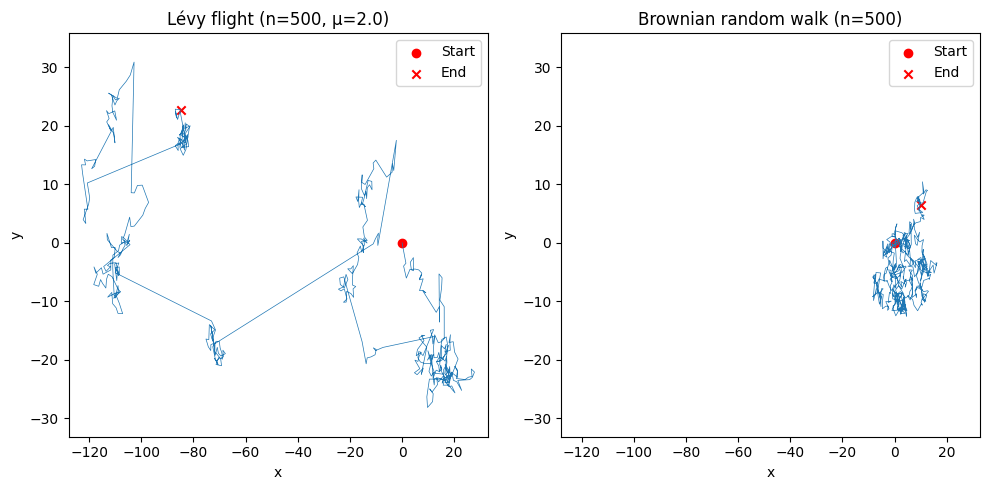
\includegraphics[width=0.9\linewidth]{images/levy_brownian.png}

    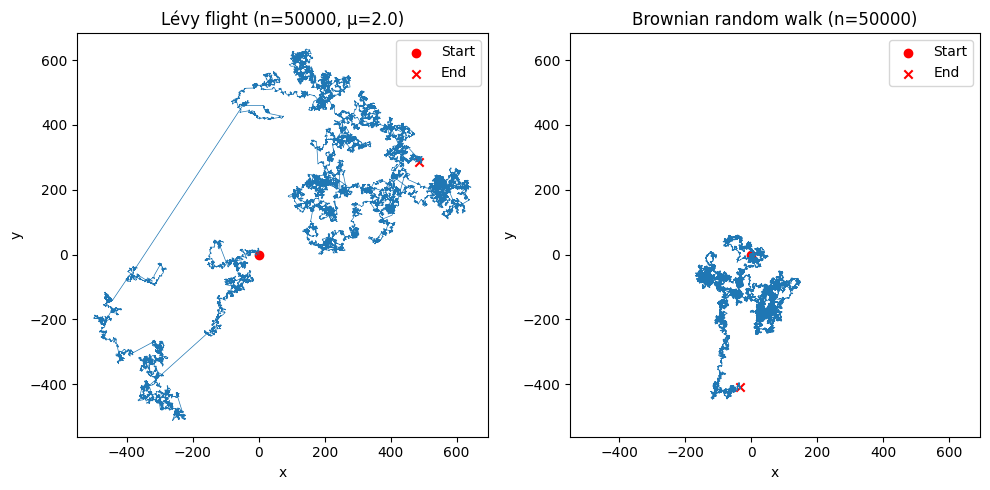
\includegraphics[width=0.9\linewidth]{images/levy_brownian1.png}
    \caption{Lévy-type (Cauchy) and Brownian trajectories of different lengths. Lévy-type paths combine many short steps with rare long relocations, while Brownian motion expands with a characteristic diffusion scale.}
    \label{fig:levy_brownian}
\end{figure}

Figure~\ref{fig:levy_brownian} contrasts a heavy-tailed trajectory and a Brownian one. Brownian motion produces strong local revisits and expands diffusively, whereas Lévy-type motion mixes local exploration with occasional long relocations. Importantly, this geometric intuition does not by itself determine optimality: in practice, the best exponent depends on (i) whether targets are depleted or revisitable, (ii) whether relocations are interrupted by detections, (iii) boundaries and finite-size effects, and (iv) whether one optimizes first-detection time or long-run encounter rate~\cite{buldyrev2021comment,levernier2020inverse,palyulin2014levy}.

\paragraph{Baseline model and why results disagree.}
A widely used baseline framework was proposed by Viswanathan \emph{et al.}~\cite{viswanathan1999optimizing}. Targets are randomly distributed in 2D; a searcher detects targets only within a finite radius $r_v$; if a target becomes visible the searcher moves to the nearest visible target; and if no target is visible the searcher chooses a random direction and a relocation length, then moves while continuously scanning within radius $r_v$. This formulation defines key parameters: detection range $r_v$, target density $\rho$, scan segment length $\Delta x$ used in simulation, finite horizon $T$ (or path budget), and the domain size and boundary conditions.

Two modeling points are especially consequential. First, the model distinguishes \emph{destructive} search (each target collected once) and \emph{nondestructive} search (targets can be revisited). In the nondestructive case, post-hit mechanics must be specified: common choices include a renewal time $\tau$ for targets or a forced departure (jump-off) distance $l_c$ from the hit target. These choices can shift, flatten, or eliminate an interior optimum in $\alpha$ and connect the model to revisitable-target and intermittent-search formulations~\cite{benichou2006twodimensional,benichou2011intermittent,lomholt2008levy,santos2004optimal}. Second, target representation in 2D is not innocuous: point targets are unrealistic because a continuous trajectory hits a point with probability zero; finite detection radius (and, effectively, finite target size) is required. Together with boundaries and discretization, such details help explain why different studies can reach contradictory conclusions, particularly when MFPT and throughput are not separated~\cite{james2011assessing,levernier2020inverse,plank2008optimal}.

\paragraph{Relevance.}
Because prior conclusions depend strongly on hidden modeling and implementation choices, a transparent and reproducible benchmark is needed to test Lévy-type optimality and to map which regimes favor which $\alpha$~\cite{edwards2007revisiting,james2011assessing,plank2008optimal}.

\paragraph{Main purpose of the research.}
The aim of this work is to construct a transparent and reproducible two-dimensional simulation benchmark for L\'evy walk search on infinite Poisson target fields, and to use this benchmark to determine---quantitatively and across a broad range of environmental and model parameters---under which conditions the inverse-square L\'evy exponent $\mu^* = 2$ is genuinely optimal, under which conditions the optimum shifts to ballistic or Brownian-like regimes, and how sensitively the optimal exponent depends on the post-detection strategy, target sparsity, and truncation parameters. Performance is evaluated using the pooled unique-capture rate and, for selected cases, the mean first-passage time (MFPT)~\cite{bartumeus2002optimizing,viswanathan1999optimizing}.

The specific research questions addressed are (stated in the
$\mu = \alpha + 1$ convention introduced in
Chapter~\ref{ch:methodology}):\phantomsection\label{sec:research_questions}
\begin{enumerate}
    \item \textbf{Existence and location of an optimum.}
    For which sparsity levels $\lambda/r_v$ and post-detection strategies does the efficiency curve $\lambda\eta(\mu)$ exhibit an interior maximum near $\mu \approx 2$ (equivalently $\alpha \approx 1$), and when does the optimum shift to the ballistic limit~\cite{buldyrev2021comment,levernier2020inverse}?
    \item \textbf{MFPT vs.\ throughput.}
    Does the exponent that minimizes MFPT coincide with the throughput-optimal exponent under identical settings~\cite{bartumeus2002optimizing,raposo2003dynamical}?
    \item \textbf{Sparsity dependence.}
    How does the optimal exponent $\mu^*$ change across two orders of magnitude in $\lambda/r_v$, and at what density does the L\'evy advantage disappear~\cite{bartumeus2005animal}?
    \item \textbf{Truncation sensitivity.}
    How do the truncation bounds $l_{\min}$ and $l_{\max}$ affect $\mu^*$ and the peak efficiency~\cite{chen2018tempered}?
    \item \textbf{Statistical convergence.}
    What number of flights and runs are required for stable estimates of $\mu^*$ and $\lambda\eta_{\max}$, particularly in the presence of trapping in non-destructive search~\cite{edwards2007revisiting,james2011assessing}?
\end{enumerate}

\paragraph{Scientific novelty.}
The novelty lies in a benchmarking methodology that makes conclusions about the optimal exponent comparable across assumptions: (i) four post-detection strategies (no-interrupt, teleport, Viswanathan destructive, Viswanathan non-destructive) are compared under identical target fields; (ii) MFPT and the pooled unique-capture rate are evaluated within the same framework; (iii) the optimal exponent $\mu^*$ (equivalently $\alpha^* = \mu^* - 1$) is mapped across two orders of magnitude in the sparsity ratio $\lambda/r_v$; and (iv) convergence studies and sensitivity analyses quantify the statistical reliability of the reported optima.

\paragraph{Statements for defense.}
\begin{enumerate}
    \item A reproducible 2D simulation framework for L\'evy walk search on an infinite Poisson target field with four post-detection strategies is implemented and validated~\cite{viswanathan1999optimizing}.
    \item The optimal L\'evy exponent converges to $\mu^* \approx 2$ ($\alpha^* \approx 1$) in the sparse-target limit for all four strategies (within the grid resolution $\Delta\mu = 0.1$), confirming the central prediction of the L\'evy foraging hypothesis.
    \item At high target density ($\lambda/r_v \leq 20$), the optimum shifts toward ballistic motion ($\mu^* = 1.0$--$1.4$) for strategies without trapping, demonstrating that L\'evy optimality is regime-dependent \cite{levernier2020inverse, bartumeus2005animal}.
    \item Non-destructive Viswanathan search exhibits pathological trapping at high density (revisit ratios $\sim 10^3$), creating spurious shifts of $\mu^*$ above~2 and necessitating pooled estimators with $R \geq 200$ runs.
\end{enumerate}

The remainder of the thesis is organized as follows.
Chapter~\ref{ch:literature_review} synthesizes evidence for and
against L\'evy-type optimality.
Chapter~\ref{ch:problem_statement} formalizes the problem and
notation.
Chapter~\ref{ch:methodology} describes the simulation methodology,
including the switch to the exponent $\mu = \alpha + 1$ used in
subsequent chapters.
Chapter~\ref{ch:experiments} presents numerical experiments:
phase diagrams of the optimal exponent, sensitivity and convergence
analyses, and comparison with analytical predictions.
Chapter~\ref{ch:discussion} summarizes results, states
conclusions, discusses limitations, and outlines possible
extensions.

%\chapter{Author contribution}
The author formulated the benchmark search model, implemented the simulator and evaluation metrics, conducted the Monte Carlo parameter sweeps, performed statistical analysis and visualization, and wrote the thesis. Supervisory guidance was provided by the academic advisor.
%\include{chapters/03_publications} % optional
\chapter{Literature review}
\label{ch:literature_review}

L\'evy search strategies lie at the intersection of ecology, statistical physics, and algorithmic search, because they provide a simple scale-free rule for exploring environments where targets are sparse and sensory information is limited. The influential model of Viswanathan \emph{et al.} suggested that inverse-square L\'evy walks (corresponding to $\alpha \approx 1$) can be near-optimal under minimal assumptions and has since become a standard reference point~\cite{viswanathan1999optimizing}. At the same time, subsequent empirical re-analyses and theoretical work have produced sharp critiques and mutually contradictory conclusions about whether $\alpha \approx 1$ is optimal in two dimensions, and even about what ``optimal'' should mean once objectives and modeling choices are specified~\cite{buldyrev2021comment,edwards2007revisiting,james2011assessing,levernier2020inverse,palyulin2014levy,plank2008optimal}. This lack of consensus motivates a systematic revisit of the classical framework and a careful separation of (i)~the modeling assumptions and (ii)~the performance criteria. Throughout this review, we use \emph{mean first-passage time (MFPT)} to the first detection and \emph{throughput} (long-run encounter rate, targets per unit distance or time) as the two main measures of performance.

This chapter first clarifies the distinction between L\'evy flights and L\'evy walks (Section~\ref{sec:flights_vs_walks}), then recalls the core Viswanathan model and its assumptions (Section~\ref{sec:core_model}), reviews results supporting L\'evy-type optimality under specific conditions (Section~\ref{sec:positive}), followed by critical and negative results that emphasize context dependence (Section~\ref{sec:negative}). Section~\ref{sec:refinements} summarizes refinements and responses that identify parameter regimes where $\alpha \approx 1$ remains strongly advantageous. Finally, Section~\ref{sec:gaps} states the outstanding questions that motivate the benchmark developed in this thesis.

%-----------------------------------------------------------
\section{L\'evy flights versus L\'evy walks}
\label{sec:flights_vs_walks}

Before reviewing the foraging literature it is important to distinguish two related but physically different stochastic models that are frequently conflated in the literature.

A \textbf{L\'evy flight} is a random walk in which the displacement at each discrete step is drawn from a heavy-tailed (power-law) distribution, and each step is completed \emph{instantaneously}---that is, every step occupies the same unit of time regardless of its length~\cite{shlesinger1986walks}. In continuous time, this means that a single step of length~$\ell$ is traversed in one time unit, implying an effective speed proportional to~$\ell$. As a consequence, L\'evy flights can produce arbitrarily large instantaneous velocities, and the mean-square displacement may diverge: the process is superdiffusive but unphysical when a finite speed is required.

A \textbf{L\'evy walk}, by contrast, is a coupled continuous-time random walk in which the walker moves at \emph{constant speed}~$v$~\cite{shlesinger1986walks,zaburdaev2015levy}. A step of length~$\ell$ takes a time $\tau = \ell/v$, so long relocations are correspondingly time-consuming. The resulting mean-square displacement is finite at any finite time (though it can still grow faster than diffusion), and the velocity is bounded. L\'evy walks are therefore the physically appropriate model for organisms or robots moving through space, which is why the foraging literature overwhelmingly studies constant-speed motion~\cite{viswanathan1999optimizing,bartumeus2005animal}.

\begin{figure}[htb]
\centering
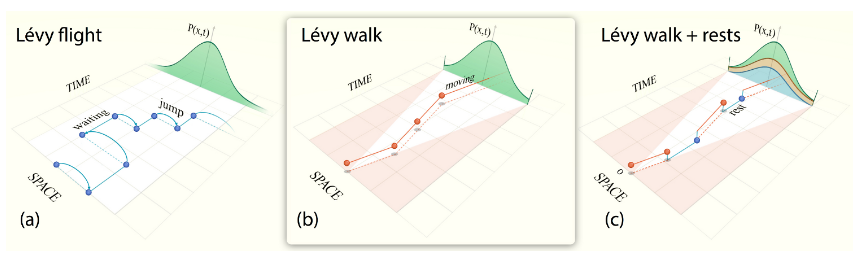
\includegraphics[width=0.85\textwidth]{images/levy_walks.png}
\caption{Schematic comparison of (a)~a L\'evy flight, in which each step is completed instantaneously (``jump''), (b)~a L\'evy walk, in which the walker moves at constant speed between turning points, and (c)~a L\'evy walk with rests, where the walker pauses at each turning point before resuming.  The upper curves show the propagator $P(x,t)$ at a fixed time.  Adapted from Zaburdaev et~al.~\cite{zaburdaev2015levy}.}
\label{fig:levy_walks}
\end{figure}

Despite this clear conceptual distinction, many publications in the foraging literature use the term ``L\'evy flight'' when the underlying model is in fact a constant-speed walk~\cite{viswanathan1999optimizing,bartumeus2002optimizing,edwards2007revisiting}. The confusion was noted already by Shlesinger and Klafter in the original chapter that introduced the terminology~\cite{shlesinger1986walks}, and persists in recent work. In this thesis, the simulation is a L\'evy \emph{walk}: the searcher moves at constant unit speed and each flight of length~$\ell$ takes time~$\ell$. Where we use the phrase ``L\'evy flight'' (following common usage in the foraging community), it should be understood as referring to this constant-speed process, not to instantaneous jumps.

%-----------------------------------------------------------
\section{Core foraging model and assumptions}
\label{sec:core_model}
The L\'evy foraging hypothesis was formalized by Viswanathan \emph{et al.} in a minimal random search model in $d=1,2$ with homogeneous target fields, constant speed, finite detection radius $r_v$, and no memory beyond immediate detection~\cite{viswanathan1999optimizing}. The model builds on earlier ideas from fractals and anomalous transport~\cite{mandelbrot1967coast,shlesinger1986walks,shlesinger1993strange} and on early empirical reports of scale-free movement patterns~\cite{cole1995fractal,focardi1996ungulates,heinrich1979resource,viswanathan1996albatross}. Step lengths are drawn from a power law
\[
P(\ell) \propto \ell^{-\mu},\quad \mu>1,
\]
which corresponds to a L\'evy-stable index $\alpha=\mu-1$.

The Viswanathan model specifies a searcher that executes a sequence of straight-line flights in uniformly random directions. When the searcher passes within a detection radius~$r_v$ of a target, it registers a detection. Two interaction modes are considered: \emph{destructive} search (each target is removed upon detection) and \emph{nondestructive} search (targets persist and may be revisited). In the destructive setting, Viswanathan \emph{et al.} derived an asymptotic expression for the mean number of flights~$N$ required per detection, $N \sim (\lambda/r_v)^{(\mu-1)/2}$, where $\lambda = 1/(2\rho r_v)$ is the mean free path~\cite{viswanathan1999optimizing}. The throughput objective is $\eta = 1/(N\langle\ell\rangle)$, where $\langle\ell\rangle$ is the mean flight length. Under their idealized assumptions (sparse targets in an effectively infinite homogeneous domain, no drift, and a particular treatment of revisits), both the destructive and the nondestructive cases in 2D exhibit an interior optimum at $\mu \simeq 2$ (equivalently $\alpha \simeq 1$). The nondestructive advantage is more pronounced because revisits additionally penalize short-range (Brownian-like) strategies that remain in the neighborhood of already-detected targets~\cite{viswanathan1999optimizing}. Numerical experiments on periodic domains confirmed these asymptotic predictions~\cite{viswanathan1999optimizing}.

Viswanathan \emph{et al.} also fitted heavy-tailed or exponential models to GPS movement data for albatrosses, deer, and bumblebees and reported $\mu \approx 2$ in large open environments, with more exponential-like behavior in confined settings~\cite{focardi1996ungulates,heinrich1979resource,viswanathan1996albatross,viswanathan1999optimizing}. This empirical component attracted widespread attention, although later re-analyses argued that such fits are statistically fragile and sensitive to data processing choices (see Section~\ref{sec:negative})~\cite{edwards2007revisiting,james2011assessing,plank2008optimal}.

\begin{figure}[htb]
\centering
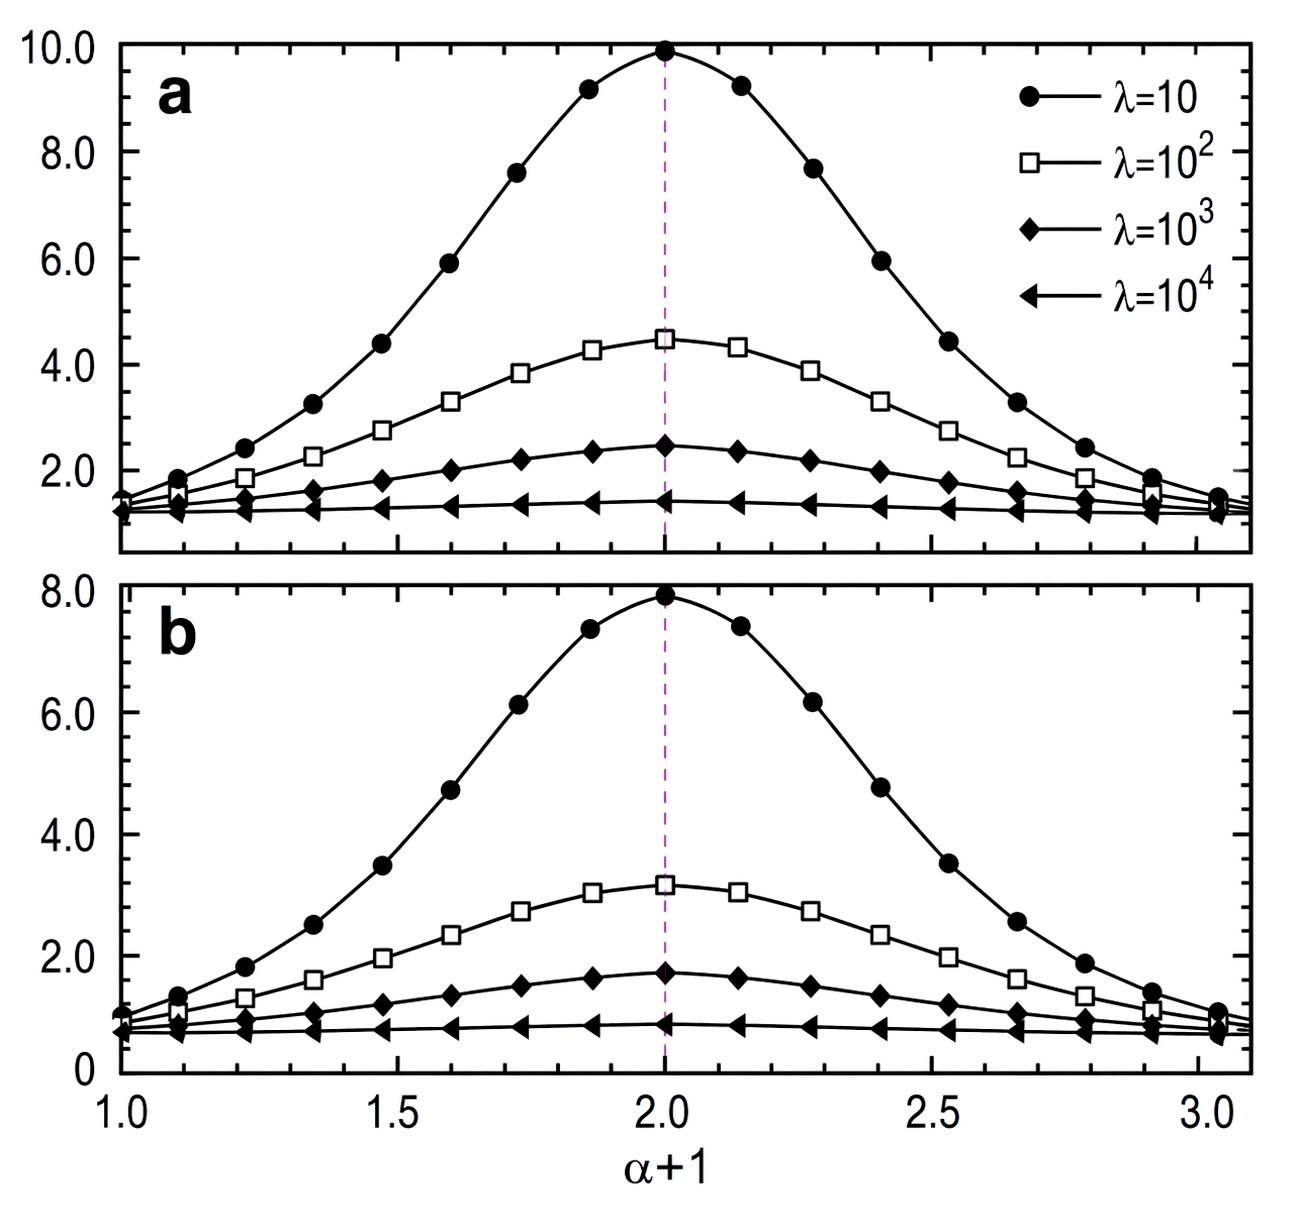
\includegraphics[width=0.5\linewidth]{images/viswanathan1999.png}
\caption{The product of the mean free path~$\lambda$ and the foraging efficiency~$\eta$ plotted against the L\'evy parameter $\alpha+1$ (reproduced from the original Viswanathan~et~al.\ (1999) paper~\cite{viswanathan1999optimizing}). The peak at $\mu \approx 2$ in the nondestructive case is the central prediction of the L\'evy foraging hypothesis.}
\label{fig:viswanathan_original}
\end{figure}

The classical framework therefore implicitly fixes several design choices: (i)~dimension~$d$; (ii)~destructive vs.\ nondestructive interactions; (iii)~boundary conditions and finite-size effects; (iv)~the performance objective (throughput vs.\ MFPT); and (v)~the specific mechanism by which nondestructive revisits are handled (e.g., renewal time, jump-off distance, or immediate restart). Much of the later literature can be read as asking what happens when one (or several) of these assumptions is changed.

%-----------------------------------------------------------
\section{Evidence in favor of L\'evy-type optimality}
\label{sec:positive}
A substantial body of work supports the claim that L\'evy-like dynamics can be efficient search strategies under clearly stated conditions. We organize these results by the type of evidence: theoretical and numerical analyses in controlled models, empirical fits to animal movement data, and evolutionary arguments.

\paragraph{Theoretical and numerical analyses.}
Bartumeus \emph{et al.}~\cite{bartumeus2002optimizing} compared L\'evy and Brownian walkers searching for randomly placed targets in continuous 1D and 2D domains. Using throughput-based performance metrics, they demonstrated that heavy-tailed relocations reduce the probability of local oversampling (repeatedly scanning already-cleared areas) and improve encounter rates for sparse targets. Their numerical simulations showed optimal exponents near $\mu \simeq 2$ in 2D, consistent with the Viswanathan prediction, and importantly highlighted that the advantage arises from the balance between local exploration (short flights) and long-range relocation (occasional ballistic segments). Raposo \emph{et al.}~\cite{raposo2003dynamical} extended this analysis to probe the dynamical robustness of the L\'evy advantage. They showed that the efficiency peak near $\mu = 2$ is not an artifact of a single parameter choice but persists under moderate perturbations of the target density and domain size. However, they also noted that the peak broadens and flattens as the environment becomes denser, foreshadowing the density dependence studied in detail in this thesis.

For revisitable targets, Santos \emph{et al.}~\cite{santos2004optimal} introduced explicit nondestructive mechanics through a renewal time~$\tau$ and a restart distance~$l_c$ in effectively unbounded 1D settings. Their key result is a two-parameter phase diagram: the preferred exponent drifts toward $\mu \to 2$ as renewal becomes fast ($\tau \to 0$) and restart distances become small ($l_c \to 0$), and toward $\mu \to 1$ (ballistic) as renewal becomes slow ($\tau \gg 1$). Intermediate regimes exhibit smooth crossovers, indicating that ``$\alpha \approx 1$ optimality'' corresponds to a specific corner of a larger parameter space rather than a universal law.

A different but closely related line of work studies \emph{intermittent search}, where the searcher alternates between a slow detection phase and a fast relocation phase without detection. B{\'e}nichou \emph{et al.}~\cite{benichou2006twodimensional} derived MFPT-optimal switching rules for intermittent searchers in 2D confined domains and showed that long relocations can substantially reduce MFPT in sparse regimes. Their comprehensive review~\cite{benichou2011intermittent} synthesizes these results across dimensions and geometries, clarifying that the advantage of intermittent strategies over purely diffusive exploration is largest when the ratio of domain size to detection radius is large---analogous to the sparse-target condition in the foraging literature. Lomholt \emph{et al.}~\cite{lomholt2008levy} further argued that L\'evy-like relocations can be advantageous within intermittent processes, provided the relocation phase duration is drawn from a heavy-tailed distribution. They showed that in certain regimes the MFPT scales as $T \sim L^{d_w}$ with a walk dimension $d_w < 2$, outperforming both ballistic and Brownian intermittent strategies.

Several extensions examine modifications of L\'evy motion itself. Chen \emph{et al.}~\cite{chen2018tempered} studied \emph{tempered L\'evy flights}, in which the power-law tail is exponentially damped beyond a characteristic scale. They showed that an optimal tempering level exists for MFPT-based search, interpolating between heavy-tailed motion (efficient exploration of distant regions) and effectively short-tailed motion (efficient local scanning). The optimal tempering scale is related to the typical inter-target distance, providing a connection to the truncation parameters ($l_{\min}$, $l_{\max}$) studied in this thesis. Padash \emph{et al.}~\cite{padash2022asymmetric} analyzed asymmetric (skewed) L\'evy flights and reported that controlled asymmetry can reduce MFPT compared to symmetric L\'evy and Brownian cases in 1D settings, suggesting that directional bias can complement the advantages of heavy-tailed relocation.

\paragraph{Empirical evidence.}
On the empirical side, Humphries \emph{et al.}~\cite{humphries2012foraging} analyzed high-resolution tracking data from 55 marine predators (including sharks, tuna, and ocean sunfish) using rigorous maximum-likelihood model selection. They reported that truncated power-law models outperformed exponential alternatives for the majority of individuals, with inferred exponents clustering near $\mu \approx 2$ during search phases in open water but shifting toward exponential behavior during area-restricted search near prey patches. Garg and Kello~\cite{garg2021efficient} documented similar L\'evy-like patterns in virtual human foraging experiments, where participants searching for hidden targets in featureless environments spontaneously adopted heavy-tailed movement strategies. Reynolds \emph{et al.}~\cite{reynolds2018rural} extended these findings to rural human foragers (Juchit\'an de Zaragoza, Mexico), reporting truncated power-law step-length distributions with $\mu \approx 2$ during mushroom and firewood collection in low-density environments. However, the inferred exponents depend on segmentation methods and the candidate model class, so these empirical results should be interpreted with appropriate caveats (see Section~\ref{sec:negative}).

\paragraph{Evolutionary arguments.}
Wosniack \emph{et al.}~\cite{wosniack2017evolutionary} used evolutionary simulations in which foraging efficiency (throughput) determined reproductive fitness. Starting from random initial exponents, populations evolving under sparse-resource conditions on periodic domains repeatedly converged to heavy-tailed exponents near $\mu \approx 2$, suggesting that L\'evy-like motion can be an evolutionarily stable strategy under a Viswanathan-style set of assumptions. The evolutionary stability lends additional theoretical support but also inherits the same model dependence: the selected exponent depends on the fitness function, boundary conditions, and target dynamics.

\paragraph{Summary.}
Under their stated assumptions (typically homogeneous domains, weak or no bias, sparse targets, and a fixed objective such as MFPT or throughput), these works collectively demonstrate that L\'evy-type strategies can outperform Brownian motion in low-information search. The advantage is most robust when targets are sparse, the searcher has no memory or cues, and the performance objective penalizes local oversampling. This motivates the central questions of this thesis (Section~\ref{sec:research_questions}): when does an interior optimum near $\alpha \approx 1$ exist in 2D, and how sensitive is it to sparsity and scale parameters?

%-----------------------------------------------------------
\section{Negative and contradictory results}
\label{sec:negative}
In contrast, several influential works question the universality of L\'evy optimality and emphasize strong context dependence. These critiques fall into three categories: empirical re-analyses, theoretical counter-examples in modified environments, and fundamental scaling arguments.

\paragraph{Empirical re-analyses.}
The most influential empirical critique came from Edwards \emph{et al.}~\cite{edwards2007revisiting}, who re-analyzed the same albatross, bee, and deer tracking datasets that had been used to support the L\'evy foraging hypothesis. Using higher-resolution data and rigorous likelihood-based model selection (Akaike information criterion and log-likelihood ratio tests), they showed that exponential-tailed alternatives (including composite Brownian models with two characteristic scales) can outperform pure power-law fits for the albatross and deer data. Critically, they demonstrated that pooling movement data across individuals---a practice common in early L\'evy analyses---can produce spurious apparent scaling: if different individuals move with different characteristic speeds, the pooled step-length distribution can mimic a power law even when each individual's distribution is exponential. This methodological critique prompted the development of more rigorous statistical frameworks. Plank and James~\cite{plank2008optimal} formalized a likelihood-based testing framework specifically designed to distinguish L\'evy walks from composite Brownian models, accounting for truncation effects and finite sample sizes. James \emph{et al.}~\cite{james2011assessing} extended this approach and applied it to multiple empirical datasets, often finding that composite Brownian or truncated exponential models provided better fits than L\'evy models. These results do not rule out heavy tails, but they substantially weaken the claim that empirical movement data robustly supports exact L\'evy laws, and they highlight the importance of per-individual analysis and proper model selection.

\paragraph{Theoretical counter-examples.}
Palyulin \emph{et al.}~\cite{palyulin2014levy} considered environments with drift (external flows or biased motion) and showed that L\'evy flights do not necessarily minimize MFPT once bias is present. In a 1D absorbing-boundary problem with constant drift, they found that for weak drift, L\'evy flights with $\alpha < 2$ can still outperform Brownian motion, but as the drift strength increases, a crossover occurs: Brownian motion becomes optimal for intermediate drift, and ballistic motion becomes optimal for strong drift. In 2D, the interaction between drift direction and the isotropic L\'evy relocation produces even more complex behavior, and the optimal strategy depends on the relative magnitudes of drift, detection radius, and inter-target distance. Volpe and Volpe~\cite{volpe2017topography} studied active particles in structured 2D landscapes with varying topography (rugged potential energy surfaces). They demonstrated that environmental heterogeneity can shift the MFPT-optimal strategy toward more local, Brownian-like exploration, because long ballistic flights in rugged landscapes are frequently interrupted by barriers, negating the advantage of superdiffusive exploration.

\paragraph{Fundamental scaling critique.}
A direct theoretical challenge to ``universal $\alpha \approx 1$ optimality in 2D'' was given by Levernier \emph{et al.}~\cite{levernier2020inverse} for destructive search in $d\ge2$. Using a first-passage approach, they derived asymptotic encounter-rate scaling and showed that, in $d\ge2$, the throughput scales linearly with target density $\rho$ for \emph{all} $\alpha\in(0,2)$: $\eta \sim C(\alpha)\,\rho$ as $\rho \to 0$. This means that changing~$\alpha$ affects only the prefactor~$C(\alpha)$, not the functional dependence on~$\rho$, so there is no parametrically superior scaling as targets become sparse. Furthermore, they showed that the prefactor~$C(\alpha)$ depends sensitively on microscopic implementation choices (cutoff scales, restart distances, detection geometry), and different choices can shift the best-performing~$\alpha$ anywhere across $(0,2)$, undermining any claim to a universal optimum in $d\ge2$. This stands in contrast to the 1D case, where the scaling exponent itself depends on~$\alpha$ and produces a genuine scaling advantage.

\paragraph{Recent critique: model artefact argument.}
Most recently, Pyke \emph{et al.}~\cite{pyke2026artefact} argued that the L\'evy foraging hypothesis is a ``model artefact.'' Through computer simulations of the standard Viswanathan model, they identified two artefactual processes that both intensify as~$\mu$ increases from~1 to~3: (i)~an increase in quick immediate revisits to food locations that happen to be near one another (revisits occurring after few intervening steps with no intervening visits to other targets), and (ii)~an increase in path resurveying (the walker repeatedly scanning previously explored territory). Pyke \emph{et al.} argued that these two processes are responsible for the decline in efficiency at $\mu > 2$, and that slight modeling modifications---such as preventing immediate revisits or penalizing path overlap---can eliminate or shift the efficiency peak, thereby removing the apparent optimality at $\mu = 2$. This critique reinforces the call to interpret L\'evy optimality as contingent on specific model rules rather than as a robust property of random search.

\paragraph{Summary.}
Overall, these results challenge three pillars of the classical hypothesis: robustness of empirical power-law fits~\cite{edwards2007revisiting,james2011assessing,plank2008optimal}, optimality in biased or structured environments~\cite{palyulin2014levy,volpe2017topography}, and universality of an $\alpha\simeq 1$ optimum in 2D~\cite{levernier2020inverse,pyke2026artefact}. Importantly, critical studies typically focus on a single objective (often MFPT or a related asymptotic scaling) and rarely compare MFPT and long-run throughput side by side under identical assumptions. This motivates a unified framework that can systematically vary assumptions and evaluate both objectives.

%-----------------------------------------------------------
\section{Refinements and responses}
\label{sec:refinements}
Several works attempt to reconcile supportive and critical results by identifying regimes where L\'evy-type strategies remain sharply advantageous.

Buldyrev \emph{et al.}~\cite{buldyrev2021comment} responded directly to the Levernier \emph{et al.} critique~\cite{levernier2020inverse} by focusing on a nondestructive ``hide-and-seek'' limit in 2D, where targets are immediately revisitable and the restart distance is close to the detection radius. Introducing the parameter $\delta = l_c/r_v - 1$ and analyzing the limit $\delta \to 0$, they showed that the encounter rate develops a sharp maximum at $\alpha=1$ ($\mu = 2$), with the relative gain of the optimal exponent over other exponents growing as~$\delta$ decreases. Specifically, the ratio $\eta(\alpha=1)/\eta(\alpha=0.5)$ increases from approximately~1.05 at $\delta = 1$ to over~1.5 at $\delta = 0.01$, demonstrating that the ``model-dependent prefactor'' identified by Levernier \emph{et al.} can be substantial in physically relevant regimes. At the same time, their analysis also highlights that this is a singular regime: for fixed $\delta>0$ the optimum can flatten and become sensitive to microscopic details (grid resolution, boundary effects, the precise detection mechanism), consistent with the broader message of model dependence.

The Bartumeus \emph{et al.}~\cite{bartumeus2005animal} review provided an important synthesis by identifying the ecological conditions under which L\'evy-type search is expected to be advantageous. They argued that L\'evy optimality requires three conditions to hold simultaneously: (1)~targets must be sparse relative to the detection radius, (2)~the searcher must have no information about target locations beyond immediate detection, and (3)~the environment must be spatially homogeneous at the scale of individual flights. When any of these conditions is violated---for example, if the forager can remember previously visited locations, or if targets are clustered---the L\'evy advantage diminishes or disappears. This framework provides a principled way to understand why different studies reach different conclusions: the disagreements reflect genuinely different parameter regimes rather than methodological errors.

A complementary direction replaces fixed power-law rules with \emph{learned} strategies. Mu{\~n}oz-Gil \emph{et al.}~\cite{munozgil2023optimal} trained reinforcement-learning agents on sparse-target environments matching the Viswanathan setup and showed that the learned policies can match or slightly exceed the efficiency of the best L\'evy exponent, achieving efficiency gains of 5--15\% over the optimal power-law walker. Kaur \emph{et al.}~\cite{kaur2023adaptive} and Caraglio \emph{et al.}~\cite{caraglio2024learning} extended this approach to active Brownian particles with intermittent strategies, showing that learned switching policies outperform fixed L\'evy exponents, particularly in heterogeneous environments. These results suggest that power-law motion, while near-optimal within its parametric family, is not globally optimal: adaptive strategies that incorporate even rudimentary memory or state information can do better. This motivates a direct comparison between optimized L\'evy flights and adaptive agents (see Chapter~\ref{ch:discussion}, Future work).

%-----------------------------------------------------------
\section{Outstanding questions and motivation for the present study}
\label{sec:gaps}
Across the analytical and empirical work reviewed in Sections~\ref{sec:positive}--\ref{sec:refinements}, the following picture emerges:
\begin{enumerate}
    \item Under idealized assumptions (typically homogeneous domains, weak bias, and carefully specified nondestructive mechanics), Lévy-type motion can maximize throughput or minimize MFPT, and in special limits $\alpha \simeq 1$ becomes sharply optimal~\cite{buldyrev2021comment,raposo2003dynamical,santos2004optimal,viswanathan1999optimizing}.
    \item Once more realistic features are included—finite domains, drift, heterogeneous landscapes, explicit renewal rules, or statistical constraints on empirical fits—the advantage can shrink to constant factors, the best exponent loses universality, and Brownian or ballistic strategies can become preferable in parts of parameter space~\cite{edwards2007revisiting,james2011assessing,levernier2020inverse,palyulin2014levy,plank2008optimal,volpe2017topography}.
\end{enumerate}

What is still missing is a minimal, fully specified 2D computational benchmark in which (a) destructive and nondestructive cases and post-hit departure rules are explicit parameters; (b) MFPT and throughput are both measured under identical settings; and (c) uncertainty is assessed (variance, convergence envelopes) so that claims about the shape and location of an optimum in $\alpha$ are reproducible. The present thesis constructs such a benchmark and uses it to map how the optimal $\alpha$ depends on objectives, interaction rules, and scale parameters, rather than treating Lévy optimality as a universal property of 2D search.

\chapter{Problem statement}
\label{ch:problem_statement}

This chapter formalizes the search problem studied in this thesis, introduces the notation used throughout, and states the research goal in a precise form. The focus is on a minimal but fully specified two-dimensional model of random search with finite detection radius, in which the effect of the Lévy tail exponent $\alpha$ can be benchmarked under controlled assumptions.

%-----------------------------------------------------------
\section{Search domain, targets, and trajectory}
The searcher operates in the Euclidean plane~$\mathbb{R}^2$.
In principle, the domain may be bounded (a finite region~$\Omega$ with
periodic or reflecting boundary conditions) or unbounded.  The
implementation used in this thesis (Chapter~\ref{ch:methodology})
adopts an effectively infinite plane realized via on-demand
generation of square chunks, thereby avoiding the finite-size
and boundary effects associated with periodic domains.

Targets are distributed as a homogeneous Poisson point process
with intensity~$\rho$ (targets per unit area).  The probability
of finding exactly~$k$ targets in a region of area~$S$ is
$P(k) = (\rho S)^k e^{-\rho S}/k!$.  The expected number of
targets in any region is $\rho S$, and target positions are
independent and uniformly distributed.

A searcher moves at constant unit speed and produces a
trajectory $x(t)\in\mathbb{R}^2$ for $t\ge 0$, so that
distance and time are interchangeable.
In simulations, each flight is decomposed into segments of
length~$\Delta x$ (the scan resolution), and detections are
checked at each segment.  The total search budget is specified
as a number of flights~$N_{\mathrm{flights}}$; together with the
exponent-dependent mean flight length, this determines the total
distance traveled.

\begin{Def}[Detection event]
Fix a detection radius $r_v>0$. A target $y_i$ is detected at time $t$ if
\begin{equation}
    \|x(t)-y_i\|\le r_v .
    \label{eq:detection_condition}
\end{equation}
\end{Def}

We emphasize that the finite radius $r_v$ is essential in 2D: if targets were modeled as mathematical points and detections required exact hits, then a continuous trajectory would detect a target with probability zero. The model therefore treats targets as detectable discs of radius $r_v$ (or, equivalently, point targets with an observation radius~$r_v$).

%-----------------------------------------------------------
\section{Motion model: incremental relocations}
Between detections, the searcher executes \emph{relocations}. Each relocation begins by sampling a direction and a relocation length. Let $\theta_k \sim \mathrm{Unif}(0,2\pi)$ be an independent heading angle, and let $\ell_k>0$ be the relocation length sampled from a parameterized family of heavy-tailed laws. The searcher then moves toward the point
\begin{equation}
    x_k^{\star} = x(t_k) + \ell_k \, (\cos\theta_k,\sin\theta_k),
    \label{eq:relocation_target_point}
\end{equation}
but the motion is \emph{incremental}: the flight is decomposed into segments of length~$\Delta x$, and the detection condition~\eqref{eq:detection_condition} is checked along each segment.  Thus relocations can be \emph{interrupted} by detections before the planned length $\ell_k$ is completed.  (In subsequent chapters, we use ``flight'' as a synonym for ``relocation.'')

\begin{Def}[Heavy-tailed L\'evy relocation family]
Fix $\alpha\in(0,2)$. A relocation distribution is called L\'evy-type if it has a power-law tail
\begin{equation}
    \Pr(\ell > s)\sim C\, s^{-\alpha}\qquad \text{as } s\to\infty,
    \label{eq:levy_tail}
\end{equation}
for some constant $C>0$. In practice, simulations use a truncated version on $[l_{\min}, l_{\max}]$ to ensure a finite mean flight length and well-defined sampling.
\end{Def}

For comparison baselines, the same incremental motion rule is used with alternative choices of relocation lengths:
\begin{itemize}
    \item \textbf{Brownian-like baseline:} short-tailed relocation lengths (e.g., exponential or Gaussian);
    \item \textbf{Ballistic baseline:} very long relocations (effectively $\alpha\to 0$ or $\mu\to 1$ in power-law notation), producing long straight runs.
\end{itemize}

%-----------------------------------------------------------
\section{Target interaction rules}
The model distinguishes two interaction regimes.

\begin{Def}[Destructive targets]
In destructive search, each target can be detected at most once. After the first detection of $y_i$, the target is removed from the active set for the remainder of the simulation.
\end{Def}

\begin{Def}[Nondestructive targets with explicit post-hit rule]
In nondestructive search, targets may be revisited. To avoid an ill-posed “stay forever” behavior, a post-hit departure mechanism is specified explicitly. Two common choices are:
\begin{enumerate}
    \item \textbf{Depletion/renewal time} $\tau \ge 0$: after a detection, the target is inactive for time $\tau$ and becomes detectable again afterwards.
    \item \textbf{Jump-off distance} $l_c>0$: after a detection, the searcher is repositioned to a point at distance $l_c$ from the target (in a random direction), ensuring departure. It is convenient to use the dimensionless parameter
    \begin{equation}
        \varepsilon := \frac{l_c}{r_v}-1 .
        \label{eq:epsilon_jumpoff}
    \end{equation}
\end{enumerate}
\end{Def}

These interaction rules are treated as first-class model parameters
rather than hidden implementation details, because they can change
qualitative conclusions about optimality.  In the implementation
(Chapter~\ref{ch:methodology}), the teleport strategy uses
$\varepsilon = 4$ ($l_c = 5\,r_v$), while the non-destructive
Viswanathan restart corresponds to the singular limit
$\varepsilon \to -1$ ($l_c \to 0$); in this limit, a minimal
``just-visited'' flag prevents the forager from re-detecting
the same target on the immediately following flight step
(see Chapter~\ref{ch:methodology} for details).

%-----------------------------------------------------------
\section{Performance criteria}
Let $\{t_j\}_{j\ge 1}$ be the (random) sequence of detection times during a run.

\begin{Def}[Mean first-passage time (MFPT)]
The mean first-passage time is the expected total distance
traveled before the first detection (equivalent to time because
the searcher moves at constant unit speed):
\begin{equation}
    \mathrm{MFPT} := \mathbb{E}[D_{\mathrm{first}}],
    \label{eq:mfpt}
\end{equation}
where $D_{\mathrm{first}}$ is the path length from the start of a
run to the first detection, and the expectation is taken over random
relocations and target placements.  The acronym MFPT follows
standard usage~\cite{viswanathan1999optimizing}.
\end{Def}

\begin{Def}[Unique-capture rate]
Over $R$ independent runs, the \emph{pooled}
unique-capture rate is defined as
\begin{equation}
    \eta := \frac{\sum_{r=1}^{R} N_{\mathrm{unique}}^{(r)}}
                 {\sum_{r=1}^{R} D_{\mathrm{total}}^{(r)}},
    \label{eq:eta_formal}
\end{equation}
where $N_{\mathrm{unique}}^{(r)}$ is the number of distinct
targets found in run~$r$ and $D_{\mathrm{total}}^{(r)}$ is the
total distance traveled.  This pooled estimator is preferred over
the per-run mean because it is robust to heavy-tailed runs
(see Chapter~\ref{ch:methodology}).  The dimensionless form is
$\lambda\eta$, where $\lambda = 1/(2\rho r_v)$ is the mean free
path.
\end{Def}

In addition to mean performance, robustness is quantified by the
dispersion of outcomes across independent runs and by convergence
studies with respect to the number of flights and runs.

%-----------------------------------------------------------
\section{Formal goal of the study}
The study aims to build a transparent numerical benchmark and, within it, to identify which Lévy exponent is optimal across regimes.

\begin{Def}[Parameter space]
Let $\Theta$ denote the set of environmental, numerical, and
interaction parameters:
\begin{equation}
    \Theta := \bigl\{\rho,\; r_v,\; l_{\min},\; l_{\max},\;
    \Delta x,\; N_{\mathrm{flights}},\;
    \mathrm{strategy}\bigr\}.
    \label{eq:parameter_space}
\end{equation}
Here \emph{strategy} takes one of four values: no-interrupt,
teleport, Viswanathan destructive, or Viswanathan non-destructive.
The key dimensionless control parameter is the sparsity ratio
$\lambda/r_v = 1/(2\rho r_v^2)$.  Note that the no-interrupt
strategy is inherently destructive (each target is counted at
most once).
\end{Def}

\begin{Def}[Objective-dependent optimal exponent]
Fix a choice of objective $\mathcal{J}\in\{\mathrm{MFPT},\, \eta\}$
and fix parameters $\theta\in\Theta$. The objective-dependent
optimal exponent is
\begin{equation}
    \alpha^\star(\theta;\mathcal{J}) \in \arg\max_{\alpha\in(0,2)}
    \, \mathcal{J}(\alpha;\theta),
    \label{eq:alpha_star}
\end{equation}
where for MFPT the maximization is replaced by minimization.
Equivalently, in the $\mu$-convention
(Chapter~\ref{ch:methodology}), $\mu^* = \alpha^* + 1$.
\end{Def}

\paragraph{Overall purpose (formal statement).}
For each regime $\theta\in\Theta$, the purpose of this thesis
is to:
\begin{enumerate}
    \item implement a reproducible 2D simulator on an infinite
          plane with Poisson-distributed targets and four
          post-detection strategies;
    \item estimate $\mathrm{MFPT}(\mu;\theta)$ and
          $\lambda\eta(\mu;\theta)$ via Monte Carlo simulation;
    \item determine $\mu^*(\theta;\mathcal{J})$ for both
          objectives and assess convergence with respect to the
          number of flights and runs;
    \item map the dependence of $\mu^*$ on the sparsity ratio
          $\lambda/r_v$ across two orders of magnitude and on the
          truncation parameters $l_{\min}/r_v$ and
          $l_{\max}/\lambda$.
\end{enumerate}

\paragraph{Problem statement (one sentence).}
Given a two-dimensional random search model on an infinite Poisson
target field with finite detection radius and explicit
post-detection strategies, determine---by systematic Monte Carlo
simulation---how the optimal L\'evy exponent $\mu^*$ depends on
the sparsity ratio $\lambda/r_v$, the truncation parameters, and
the choice of strategy.

% ============================================================
%  Chapter 4 — Methodology
% ============================================================
\chapter{Methodology}
\label{ch:methodology}

%-------------------------------------------------------------
\section{Mathematical model}
\label{sec:math_model}

\subsection{Target field}

Targets are distributed in the Euclidean plane $\mathbb{R}^2$ as
a homogeneous Poisson point process (PPP) with intensity~$\rho$
(number of targets per unit area).  The probability of finding
exactly~$k$ targets in a region of area~$S$ is
\begin{equation}
  P(k) = \frac{(\rho S)^k}{k!}\,e^{-\rho S}.
  \label{eq:poisson}
\end{equation}
The PPP is memoryless and isotropic: target positions are
independent, and any subregion has the same statistical
properties.  The mean nearest-neighbor distance is
$\langle d_{\mathrm{nn}} \rangle = 1/(2\sqrt{\rho})$.

\subsection{L\'evy flight}

\paragraph{Notation.}
In the preceding chapters, the tail exponent was denoted $\alpha\in(0,2)$,
with the survival function $\Pr(\ell > s)\sim C\,s^{-\alpha}$.
Following Viswanathan et~al.~\cite{viswanathan1999optimizing}, we now switch
to the exponent $\mu:=\alpha+1$, so that $\mu\in(1,3)$ and
$P(\ell)\propto\ell^{-\mu}$.  In particular, the theoretical prediction
$\alpha\approx 1$ of the L\'evy foraging hypothesis corresponds to
$\mu\approx 2$.  Both notations are common in the literature; the
$\mu$-convention is used throughout this and subsequent chapters.

A forager (searcher) moves through the target field as a
sequence of straight-line flights.  Each flight has:
\begin{itemize}
  \item a \emph{direction}~$\theta$, drawn uniformly on
        $[0,2\pi)$;
  \item a \emph{length}~$l$, drawn from the truncated power-law
        distribution~\eqref{eq:levy_pdf} below.
\end{itemize}
\begin{equation}
  p(l) = \frac{(\mu-1)\,l_{\min}^{\mu-1}}{1 - (l_{\min}/l_{\max})^{\mu-1}}\,
         l^{-\mu}, \qquad l \in [l_{\min},\,l_{\max}],
  \label{eq:levy_pdf}
\end{equation}
where $\mu > 1$ is the L\'evy exponent.  The cumulative
distribution function is
\begin{equation}
  F(l) = \frac{l_{\min}^{1-\mu} - l^{1-\mu}}
              {l_{\min}^{1-\mu} - l_{\max}^{1-\mu}},
  \qquad l \in [l_{\min},\,l_{\max}].
\end{equation}
Samples are generated by the inverse-CDF method:
\begin{equation}
  l = \bigl[l_{\min}^{1-\mu}
      + u\,(l_{\max}^{1-\mu} - l_{\min}^{1-\mu})\bigr]^{1/(1-\mu)},
  \qquad u \sim \mathrm{Uniform}(0,1),\quad \mu \neq 1.
  \label{eq:inverse_cdf}
\end{equation}
At the boundary $\mu = 1$ the normalization becomes
logarithmic and the inverse-CDF reduces to
$l = \exp\!\bigl[\ln l_{\min} + u\,(\ln l_{\max} - \ln l_{\min})\bigr]$,
i.e.\ a log-uniform distribution on $[l_{\min},\,l_{\max}]$.
The implementation detects $|\mu - 1| < 10^{-12}$ and switches
to this formula to avoid a singularity in the generic expression.

The first moment of $p(l)$ is
\begin{equation}
  \langle l \rangle = \frac{\mu-1}{\mu-2}\cdot
     \frac{l_{\max}^{2-\mu} - l_{\min}^{2-\mu}}
          {l_{\max}^{1-\mu} - l_{\min}^{1-\mu}},
  \qquad \mu \neq 2.
  \label{eq:mean_l}
\end{equation}
For $\mu = 2$: $\langle l \rangle = \ln(l_{\max}/l_{\min})
\big/ \bigl(l_{\min}^{-1} - l_{\max}^{-1}\bigr)$.
The mean length diverges as $l_{\max}\to\infty$ for $\mu \leq 2$,
which is the hallmark of L\'evy flights.

\subsection{Detection model}

During each flight segment the forager detects any target whose
distance from the flight path is at most the vision radius~$r_v$.
Geometrically, the detection zone is a rectangle (``corridor'') of
width~$2r_v$ and length equal to the segment length, plus two
semicircular endcaps of radius~$r_v$.
When multiple targets lie within detection range of a single
segment, the implementation computes the exact entry distance
(via segment--circle intersection) for each candidate target
and selects the \emph{first} target along the direction of motion.
This continuous first-hit ordering ensures that the forager
always encounters the geometrically nearest target first,
regardless of memory layout or chunk boundaries.

The mean free path --- the average distance a forager must travel
between consecutive detections in a fresh PPP field --- is
\begin{equation}
  \lambda = \frac{1}{2\,\rho\,r_v}.
  \label{eq:lambda}
\end{equation}
The dimensionless sparsity parameter
\begin{equation}
  \frac{\lambda}{r_v} = \frac{1}{2\,\rho\,r_v^2}
  \label{eq:sparsity}
\end{equation}
controls the search regime:
$\lambda/r_v \ll 1$ corresponds to dense targets (the
forager detects a target almost every step), while
$\lambda/r_v \gg 1$ corresponds to sparse targets (the
forager flies long distances between encounters).

%-------------------------------------------------------------
\section{Post-detection strategies}
\label{sec:strategies}

Upon detecting a target, the forager's behavior depends on the
chosen post-detection strategy.

\paragraph{Strategy 1: No interrupt.}
The forager registers the detection but continues along the
pre-planned flight path until the full flight length is
completed.  The next flight starts from the end of the
current one.  All distinct targets whose detection discs
are crossed during the flight are counted (each target at
most once per run, since the search is destructive for this
strategy).  This strategy represents passive detection
during undirected motion.

\paragraph{Strategy 2: Teleport.}
The flight terminates at the detection point.  The forager
is repositioned to a random point at distance~$l_c$ from the
detected target, in a uniformly random direction.
A new flight then starts from this repositioned location.
We use $l_c = 5\,r_v$ throughout.

\paragraph{Strategy 3: Viswanathan restart.}
Following Viswanathan et~al.~\cite{viswanathan1999optimizing},
the flight terminates at the target position, and a new
flight starts \emph{from the target} with a fresh random
direction and length drawn from~\eqref{eq:levy_pdf}.
Two sub-modes are considered:
\begin{itemize}
  \item \emph{Destructive} (\texttt{remove\_prob}\,$= 1$): the detected
        target is removed from the field.  Each target can be
        found at most once.
  \item \emph{Non-destructive} (\texttt{remove\_prob}\,$= 0$): targets
        remain after detection.  The forager may revisit the
        same target multiple times.
\end{itemize}

In non-destructive mode, a ``just-visited'' flag prevents the
forager from immediately re-detecting the same target on the
very next flight step, but does not prevent revisits on
subsequent flights.  This corresponds to the
limit $l_c \to 0$ ($\varepsilon \to -1$) in the notation of
Chapter~\ref{ch:problem_statement}; the just-visited flag is a
minimal substitute that breaks the degenerate zero-length cycle
while keeping the forager at the target position.

%-------------------------------------------------------------
\section{Efficiency metrics}
\label{sec:metrics}

\subsection{Pooled unique-capture rate}

The primary efficiency metric is the \emph{pooled} (global)
unique-capture rate:
\begin{equation}
  \eta = \frac{\sum_{r=1}^{R} N_{\mathrm{unique}}^{(r)}}
              {\sum_{r=1}^{R} D_{\mathrm{total}}^{(r)}},
  \label{eq:eta}
\end{equation}
where $R$ is the number of independent runs,
$N_{\mathrm{unique}}^{(r)}$ is the number of \emph{distinct}
targets found in run~$r$, and $D_{\mathrm{total}}^{(r)}$ is the
total distance traveled.  The normalized (dimensionless) form is
$\lambda\eta$.

The pooled estimator~\eqref{eq:eta} is preferred over the
per-run mean
$\bar\eta = R^{-1}\sum_r N_{\mathrm{unique}}^{(r)}/D_{\mathrm{total}}^{(r)}$
because it is robust to heavy-tailed runs where a single
short run with many detections can dominate the average.
In the pooled form, long-distance runs contribute
proportionally to their flight length, providing a
variance-weighted estimate.

\subsection{Mean first passage time (MFPT)}

The MFPT is the average distance the forager must travel to
detect the \emph{first} target:
\begin{equation}
  \mathrm{MFPT} = \left\langle D_{\mathrm{first}} \right\rangle_R,
  \label{eq:mfpt_method}
\end{equation}
where $D_{\mathrm{first}}$ is the total distance from the start
of a run to the first detection.  We normalize this as
$\mathrm{MFPT}/\lambda$ for cross-density comparisons.

%-------------------------------------------------------------
\section{Simulation algorithm}
\label{sec:algorithm}

\subsection{Infinite-plane chunked world}

The simulation operates on an infinite 2D plane, avoiding
periodic boundary conditions.  The plane is divided into
square chunks of side $\Delta_{\mathrm{chunk}}$.  Targets
within each chunk are generated from a Poisson process
seeded deterministically from the chunk coordinates and a
global world seed:
\begin{equation}
  N_{\mathrm{chunk}} \sim \mathrm{Poisson}(\rho\,\Delta_{\mathrm{chunk}}^2),
  \qquad
  (x_i, y_i) \sim \mathrm{Uniform}(\mathrm{chunk\,bounds}).
\end{equation}
This ensures reproducibility: the same world seed always
produces the same target field.  Chunks are generated lazily
--- only when the forager's trajectory enters them --- and
persist for the duration of each run, so a forager re-entering
a previously visited chunk encounters only the surviving
(non-detected) targets.

\begin{figure}[htb]
\centering
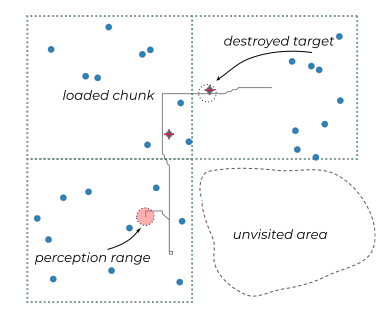
\includegraphics[width=0.55\textwidth]{images/chunks.png}
\caption{Schematic of the infinite-plane chunked world.  Square chunks (solid outlines) are loaded on demand as the forager moves; blue dots represent Poisson-distributed targets.  The perception range (dashed circle around the forager) defines the detection radius~$r_v$.  A destroyed target (crossed out) has been detected and removed in a previous flight.  The dashed region in the lower right indicates an unvisited area whose chunks have not yet been generated.}
\label{fig:chunks}
\end{figure}

\paragraph{Random number generation.}
All random variates (Poisson counts, uniform positions, flight
directions and lengths) are generated using the Mersenne Twister
(\texttt{mt19937}) seeded per-run from a master seed.
The chunk-level Poisson counts use a seed derived deterministically
from the chunk coordinates and the world seed, ensuring that
the target field is independent of the traversal order.

\subsection{Flight simulation}

For each $\mu$ value in the sweep $[\mu_{\min}, \mu_{\max}]$
with step~$\Delta\mu$:

\begin{enumerate}
  \item For each run $r = 1, \ldots, R$:
    \begin{enumerate}
      \item Initialize the forager at the origin.
            Regenerate the world (fresh PPP for each run).
      \item For each flight $n = 1, \ldots, N_{\mathrm{flights}}$:
        \begin{enumerate}
          \item Sample flight length $l \sim p(l;\mu)$ via
                \eqref{eq:inverse_cdf} and direction
                $\theta \sim \mathrm{Uniform}(0, 2\pi)$.
          \item Decompose the flight into segments of length
                $\Delta x$ (scan resolution).
          \item For each segment, load the relevant chunk and
                check all targets within detection radius~$r_v$
                of the segment centerline.
          \item Apply the post-detection strategy (no interrupt,
                teleport, or Viswanathan restart).
        \end{enumerate}
      \item Record $N_{\mathrm{unique}}^{(r)}$,
            $N_{\mathrm{visits}}^{(r)}$,
            $D_{\mathrm{total}}^{(r)}$,
            $D_{\mathrm{first}}^{(r)}$.
    \end{enumerate}
  \item Compute pooled metrics
        $\eta(\mu)$, $\lambda\eta(\mu)$, $\mathrm{MFPT}(\mu)$.
  \item Write results to CSV.
\end{enumerate}

\paragraph{Computation cost.}
A single $\mu$-sweep (21~values, $R = 120$ runs,
50\,000~flights each) completes in approximately
10--15~minutes on a single core (Intel Core~i7, 3.6\,GHz).
The full phase-diagram study (8~sparsity levels $\times$
4~strategies) required ${\sim}30$ CPU-hours in total.

\subsection{Default parameters}

\begin{table}[htb]
\centering
\begin{tabular}{llr}
\toprule
Parameter & Symbol & Default \\
\midrule
Vision radius         & $r_v$           & $0.5$ \\
Min flight length     & $l_{\min}$      & $r_v = 0.5$ \\
Max flight length     & $l_{\max}$      & $\lambda$ \\
Scan segment length   & $\Delta x$      & $50$ (in units of $r_v$: $100\,r_v$) \\
Chunk side            & $\Delta_{\mathrm{chunk}}$ & $2000$ \\
Teleport distance     & $l_c$           & $5\,r_v = 2.5$ \\
$\mu$ sweep           & $\mu_{\min}$--$\mu_{\max}$ & $1.0$--$3.0$ \\
$\mu$ step            & $\Delta\mu$     & $0.1$ \\
\bottomrule
\end{tabular}
\caption{Default simulation parameters.  The choice $r_v = 0.5$
         gives $\lambda = 1/\rho$, simplifying bookkeeping; all
         results are reported in dimensionless form
         ($\lambda/r_v$, $\lambda\eta$), so the particular value
         of~$r_v$ does not affect conclusions.}
\label{tab:defaults}
\end{table}

The density-dependent parameters (flights per run, number of runs)
vary with $\lambda/r_v$; see Table~\ref{tab:phase_params}
in Chapter~\ref{ch:experiments} for exact values.  As a rule,
$N_{\mathrm{flights}}$ ranges from 20\,000 (dense) to 150\,000
(sparse), and $R$ ranges from 100 to 120 for destructive and
300 to 360 for non-destructive strategies.

\paragraph{Scan resolution.}
The scan segment length $\Delta x = 50$ is much larger than
$r_v = 0.5$, but this does not cause missed detections: the
detection model checks whether any target center lies within
distance~$r_v$ of the straight-line segment, using the full
corridor geometry (rectangle of width~$2r_v$ plus endcaps).
Thus $\Delta x$ controls the frequency of chunk lookups, not
the detection fidelity.  To verify this, a comparison run was
performed at $\lambda/r_v = 100$ (destructive Viswanathan,
$\mu = 2.0$, $R = 50$) with $\Delta x = r_v = 0.5$: the
resulting $\lambda\eta = 0.469$ vs.\ $0.470$ with
$\Delta x = 50$, a relative difference of~$0.2\%$.

\paragraph{Flight budget.}
The search budget is specified as a fixed number of
flights~$N_{\mathrm{flights}}$ rather than a fixed total
distance.  Because the mean flight length $\langle l \rangle$
varies with~$\mu$, this means different $\mu$ values yield
different total distances.  We use the pooled
estimator~\eqref{eq:eta}, which normalizes by total distance
and is therefore invariant to this choice.  A fixed-distance
budget (terminating each run after a given distance) would
yield the same pooled~$\eta$ up to end-of-run boundary effects,
which are negligible for large $N_{\mathrm{flights}}$.

%-------------------------------------------------------------
\section{Truncation parameters}
\label{sec:truncation}

The standard choice $l_{\min} = r_v$, $l_{\max} = \lambda$
sets the scale of the shortest flights to the detection scale
and the longest flights to the mean free path.

To study the effect of truncation, we vary:
\begin{itemize}
  \item $l_{\max}/\lambda \in \{0.1,\,0.2,\,0.5,\,1,\,2,\,5,\,10\}$
        with fixed $l_{\min} = r_v$;
  \item $l_{\min}/r_v \in \{0.1,\,0.25,\,0.5,\,1,\,2,\,5\}$
        with fixed $l_{\max} = \lambda$.
\end{itemize}

%-------------------------------------------------------------
\section{Statistical methodology}
\label{sec:stat_method}

\subsection{Choice of runs}

The number of independent runs~$R$ for each $\mu$ value
is chosen to ensure convergence of the pooled estimator.
Convergence studies (Section~\ref{sec:convergence}) show that
$R \geq 50$ suffices for the destructive strategy, while
the non-destructive strategy requires $R \geq 200$ due to
the heavy-tailed distribution of per-run efficiency caused by
trapping.

\subsection{Optimal exponent extraction}

For each set of parameters, the optimal L\'evy exponent
$\mu^*$ is defined as the $\mu$ value that maximizes the
pooled unique-capture rate:
\begin{equation}
  \mu^* = \arg\max_{\mu} \lambda\eta(\mu).
  \label{eq:mu_star}
\end{equation}
The resolution of $\mu^*$ is limited by the $\mu$-grid step
$\Delta\mu = 0.1$.

\subsection{Uncertainty assessment}

Because the pooled estimator~\eqref{eq:eta} aggregates distance
and detections across all runs, individual error bars on
$\lambda\eta$ are not directly available from the pooled ratio.
Instead, uncertainty is assessed through convergence studies
(Section~\ref{sec:convergence}): $\lambda\eta(\mu)$ is computed
for increasing numbers of flights and runs, and the
variation of $\mu^*$ and $\lambda\eta_{\max}$ across these
subsamples quantifies the statistical stability of the results.
For the destructive strategy, $\lambda\eta_{\max}$ converges
within $0.5\%$ at $R \geq 50$.  For the non-destructive
strategy, $\mu^*$ remains noisy ($\pm 0.3$--$0.5$) even at
$R = 400$, although $\lambda\eta_{\max}$ converges within $1\%$
at $R \geq 200$.  These convergence envelopes effectively serve
as uncertainty bounds on the reported values.

%-------------------------------------------------------------
\section{Analytical benchmark}
\label{sec:analytical_theory}

As an analytical benchmark we use the mean-field model of
Viswanathan et~al.~\cite{viswanathan1999optimizing}.  The
unique-capture rate is approximated as
\begin{equation}
  \eta \;\approx\; \frac{1}{\langle l \rangle_{\mathrm{MF}}
  \cdot N(\mu)},
  \label{eq:eta_analytical}
\end{equation}
where $\langle l \rangle_{\mathrm{MF}}$ is a mean-field
mean flight distance and $N(\mu)$ is the mean number of
flights between successive target encounters.

The mean-field flight distance
(Viswanathan~et~al.\ eq.~2) treats flights longer than
$\lambda$ as contributing $\lambda$ (mean-field truncation):
\begin{equation}
  \langle l \rangle_{\mathrm{MF}} = r_v \left[
    \frac{(\mu-1)(R^{2-\mu}-1)}{2-\mu} + R^{2-\mu}
  \right], \qquad R = \lambda/r_v,\; \mu \neq 1,2.
  \label{eq:mean_l_mf}
\end{equation}
Limiting cases: $\langle l \rangle_{\mathrm{MF}} = \lambda$
for $\mu = 1$ and
$\langle l \rangle_{\mathrm{MF}} =
r_v(\ln R + 1)$ for $\mu = 2$.

The encounter scaling
(Viswanathan~et~al.\ eq.~5) gives
\begin{equation}
  N(\mu) = \left(\frac{\lambda}{r_v}\right)^{(\mu-1)/2},
  \label{eq:N_visw}
\end{equation}
so that the dimensionless efficiency is
$\lambda\eta \approx C \cdot
\lambda / (\langle l \rangle_{\mathrm{MF}} \cdot N)$,
where the proportionality constant~$C$ is fitted by
least squares to the simulation data.

\paragraph{Qualitative behavior.}
For $\mu < 2$,
$\langle l \rangle_{\mathrm{MF}}$ grows as
$R^{2-\mu}$ while $N$ is moderate, so $\eta$ decreases
toward the ballistic limit ($\mu \to 1$).
For $\mu > 2$,
$\langle l \rangle_{\mathrm{MF}}$ saturates near~$r_v$,
but $N$ grows as $R^{(\mu-1)/2}$, penalizing short-flight
strategies for trajectory self-intersection (revisiting
cleared areas).  The product
$\langle l \rangle_{\mathrm{MF}} \cdot N$ is therefore
minimized near $\mu \approx 2$, predicting the efficiency
peak at the L\'evy--Brownian transition.

\paragraph{Limitations.}
The encounter exponent~\eqref{eq:N_visw} was originally
derived for the non-destructive case; it is applied here
as an approximation to the destructive Viswanathan strategy
under the assumption that trajectory self-intersection
(the dominant correction in 2D) follows similar scaling.
The model overestimates efficiency for $\mu > 2.5$
(Section~\ref{sec:analytical_comparison}), where the
penalty for oversampling by very short flights exceeds the
$N(\mu)$ correction.
% ============================================================
%  Chapter 5 — Numerical Experiments
% ============================================================
\chapter{Numerical experiments}
\label{ch:experiments}

All simulations are implemented in~C99 (gcc, \texttt{-std=c99 -O3}),
single-threaded.
Source files: \texttt{levy\_viswanathan.c} (Viswanathan
destructive and non-destructive modes),
\texttt{levy\_no\_interrupt.c} (no-interrupt mode), and
\texttt{levy\_teleport.c} (teleport mode).
Plotting: \texttt{plot\_full\_study.py} (Python~3 / Matplotlib).
All lengths are measured in arbitrary units; we fix
$r_v = 0.5$ and express all other lengths relative to this
scale.  The source code will be archived in a public repository
(with a persistent DOI) upon thesis defense; in the interim
it is available from the author upon request.

%-------------------------------------------------------------
\section{Phase diagram: $\mu^*(\lambda/r_v)$}
\label{sec:phase_diagram}

\subsection{Experiment setup}

We construct the phase diagram by sweeping
$\lambda/r_v \in \{10, 20, 50, 100, 200, 500, 1000, 2000\}$.
For each sparsity level, we run all four strategies with
parameters given in Table~\ref{tab:phase_params}.

\begin{table}[htb]
\centering
\begin{tabular}{rccc}
\toprule
$\lambda/r_v$ & $\rho$ & Flights & Runs (destr./non-destr.) \\
\midrule
   10 & $0.200$ &  20\,000 & 100 / 300 \\
   20 & $0.100$ &  20\,000 & 100 / 300 \\
   50 & $0.040$ &  30\,000 & 100 / 300 \\
  100 & $0.020$ &  50\,000 & 120 / 360 \\
  200 & $0.010$ &  60\,000 & 120 / 360 \\
  500 & $0.004$ &  80\,000 & 120 / 360 \\
 1000 & $0.002$ & 100\,000 & 120 / 360 \\
 2000 & $0.001$ & 150\,000 & 120 / 360 \\
\bottomrule
\end{tabular}
\caption{Phase diagram parameters.  The number of flights per
         run grows with $\lambda/r_v$ to maintain
         adequate convergence at sparse densities.
         Non-destructive runs are $3\times$ the destructive
         count.}
\label{tab:phase_params}
\end{table}

\subsection{Results: optimal exponent $\mu^*$}

\begin{figure}[htb]
\centering

\includegraphics[width=0.88\textwidth]{images/phase_diagram_mu_star.pdf}
\caption{Phase diagram of the optimal L\'evy exponent $\mu^*$ as a function of the sparsity parameter $\lambda/r_v$ for all four post-detection strategies. The blue curve with circles corresponds to the no-interrupt strategy, the orange curve with squares to the teleport strategy ($l_c = 5r_v$), the red curve with upward triangles to the Viswanathan destructive strategy, and the green curve with downward triangles to the Viswanathan non-destructive strategy. The grey dashed horizontal line marks the theoretical prediction $\mu = 2$. Shaded bands indicate the $\pm 1\sigma$ uncertainty region.}
\label{fig:phase_diagram}
\end{figure}

Table~\ref{tab:mu_star_values} presents the numerical values.

\begin{table}[htb]
\centering
\small
\begin{tabular}{rcccc}
\toprule
$\lambda/r_v$ & No interrupt & Teleport & Visw.\ destr. & Visw.\ non-destr. \\
\midrule
   10 & 1.1 & 1.0 & 1.0 & 2.2 \\
   20 & 1.4 & 1.4 & 1.2 & 2.6 \\
   50 & 1.8 & 1.8 & 1.7 & 2.6 \\
  100 & 1.9 & 1.9 & 1.7 & 2.5 \\
  200 & 1.9 & 1.8 & 1.9 & 2.0 \\
  500 & 2.0 & 1.9 & 1.8 & 1.9 \\
 1000 & 2.0 & 2.0 & 1.9 & 2.0 \\
 2000 & 2.0 & 2.0 & 1.8 & 2.0 \\
\bottomrule
\end{tabular}
\caption{Optimal L\'evy exponent $\mu^*$ at each sparsity level.
         Resolution: $\Delta\mu = 0.1$.  Convergence studies
         (Section~\ref{sec:convergence}) show that $\mu^*$ is
         stable to $\pm 0.1$--$0.2$ for destructive strategies
         and $\pm 0.3$--$0.5$ for non-destructive Viswanathan.}
\label{tab:mu_star_values}
\end{table}

At $\lambda/r_v \geq 500$, all strategies yield
$\mu^* = 1.8$--$2.0$, approaching the theoretical prediction
(the residual offset is within the grid resolution and truncation
effects; see Section~\ref{sec:convergence}).
At $\lambda/r_v = 10$--$20$, three strategies (No interrupt,
Teleport, Visw.\ destructive) shift to $\mu^* \approx 1.0$--$1.4$
(ballistic regime), while non-destructive Viswanathan shows
$\mu^* \approx 2.2$--$2.6$ due to trapping bias.

\subsection{Efficiency scaling}

\begin{figure}[htb]
\centering

\includegraphics[width=0.88\textwidth]{images/efficiency_scaling.pdf}
\caption{Maximum dimensionless efficiency $\lambda\eta_{\max}$ as a function of target sparsity $\lambda/r_v$ for all four strategies. Colors and markers follow the same convention as Figure~\ref{fig:phase_diagram}. The three destructive strategies converge to a narrow band $\lambda\eta_{\max} \approx 0.36$--$0.51$ across the full sparsity range, while the non-destructive Viswanathan strategy (green, downward triangles) is severely penalized at low $\lambda/r_v$ by the trapping effect (see Section~\ref{sec:trapping}), reaching only $\lambda\eta_{\max} \approx 0.01$ at $\lambda/r_v = 10$.}
\label{fig:efficiency_scaling}
\end{figure}

\begin{table}[htb]
\centering
\small
\begin{tabular}{rcccc}
\toprule
$\lambda/r_v$ & No int. & Teleport & V.\ destr. & V.\ non-d. \\
\midrule
   10 & 0.364 & 0.323 & 0.384 & 0.010 \\
   50 & 0.441 & 0.435 & 0.458 & 0.124 \\
  100 & 0.454 & 0.458 & 0.470 & 0.222 \\
  500 & 0.495 & 0.499 & 0.502 & 0.476 \\
 2000 & 0.508 & 0.512 & 0.511 & 0.509 \\
\bottomrule
\end{tabular}
\caption{$\lambda\eta_{\max}$ at selected sparsity levels
         (intermediate values $\lambda/r_v = 20,\,200,\,1000$
         omitted for brevity; the full data are in
         Figure~\ref{fig:efficiency_scaling}).
         Values are converged to within $0.5\%$ for destructive
         strategies and $1\%$ for non-destructive
         (Section~\ref{sec:convergence}).}
\label{tab:eta_max}
\end{table}

At $\lambda/r_v = 2000$, all four strategies converge to
$\lambda\eta_{\max} \approx 0.51$: the post-detection protocol
becomes irrelevant when targets are far apart.

\subsection{Efficiency curves $\lambda\eta(\mu)$}

\begin{figure}[htb]
\centering

\includegraphics[width=\textwidth]{images/eta_curves_by_sparsity.pdf}
\caption{Dimensionless efficiency $\lambda\eta(\mu)$ at five sparsity levels, arranged from dense (top-left, $\lambda/r_v = 10$) to sparse (bottom-right, $\lambda/r_v = 2000$). Within each panel, the blue curve represents the no-interrupt strategy, the orange curve the teleport strategy, the red curve the Viswanathan destructive strategy, and the green curve the Viswanathan non-destructive strategy. Shaded bands show $\pm 1\sigma$ per-run standard deviation. At $\lambda/r_v = 10$ the curves are nearly flat (efficiency varies by less than $10\%$ across all~$\mu$), indicating that the choice of L\'evy exponent matters little when targets are abundant. At $\lambda/r_v = 2000$ a sharp peak emerges near $\mu \approx 2$ for all four strategies, confirming the L\'evy foraging hypothesis in the sparse limit.}
\label{fig:eta_curves}
\end{figure}

The shape of the $\lambda\eta(\mu)$ curves can be understood through the interplay of two competing effects. For $\mu < 2$, the mean flight length $\langle l \rangle$ grows with decreasing~$\mu$ (longer flights), which increases the distance traveled per detection attempt; efficiency therefore declines toward the ballistic limit ($\mu \to 1$). The decline on the left side of the curves reflects the increasing cost of long flights that traverse mostly empty space. For $\mu > 2$, the mean flight length saturates near~$l_{\min}$ (the searcher executes predominantly short flights), but the encounter factor $N(\mu) \sim (\lambda/r_v)^{(\mu-1)/2}$ grows, because short-flight trajectories exhibit strong self-intersection: the searcher repeatedly scans previously visited areas rather than exploring new territory. The efficiency decline on the right side of the curves reflects this oversampling penalty. The peak near $\mu \approx 2$ represents the balance point where the searcher makes flights long enough to avoid local oversampling but not so long that each flight is wasted traversing target-free space.

The second moment of the flight-length distribution, $\langle l^2 \rangle$, diverges for $\mu < 3$ in the untruncated case and is controlled by $l_{\max}$ in the truncated distribution used here. The transition at $\mu = 2$ is particularly significant because it separates the regime where $\langle l \rangle$ depends on $l_{\max}$ ($\mu < 2$, mean dominated by long flights) from the regime where $\langle l \rangle$ is determined by $l_{\min}$ ($\mu > 2$, mean dominated by short flights). This transition in the first moment, combined with the increasing oversampling penalty for $\mu > 2$, produces the cusp-like peak in the efficiency curves.

%-------------------------------------------------------------
\section{Trapping effect}
\label{sec:trapping}

In non-destructive Viswanathan mode, the forager restarts from
the target position and can immediately re-encounter nearby
targets.  This ``ping-pong'' trapping dominates at high density.

\begin{figure}[htb]
\centering

\includegraphics[width=0.88\textwidth]{images/trapping_heatmap.pdf}
\caption{Heatmap of trapping intensity for the Viswanathan non-destructive strategy, showing the ratio $V/U$ (total visits divided by unique captures) as a function of $\mu$ (horizontal axis) and $\lambda/r_v$ (vertical axis). The color scale is logarithmic (yellow--orange--red from low to high trapping). At $\lambda/r_v = 10$ the trapping ratio exceeds $10^3$ for all~$\mu$, indicating that each unique target is revisited over a thousand times on average. At $\lambda/r_v \geq 500$ the ratio drops below~2, indicating negligible trapping.}
\label{fig:trapping_heatmap}
\end{figure}

\begin{table}[htb]
\centering
\begin{tabular}{rcc}
\toprule
$\lambda/r_v$ & $V/U$ at $\mu=1.0$ & $V/U$ at $\mu=2.0$ \\
\midrule
   10 & 1540 & 1716 \\
   50 &   43 &   53 \\
  100 &   11 &   14 \\
  500 &  1.6 &  2.0 \\
 2000 &  1.0 &  1.2 \\
\bottomrule
\end{tabular}
\caption{Representative trapping ratios.  At $\lambda/r_v = 10$,
         each unique target is revisited ${\sim}1500$ times.}
\label{tab:trapping_ratios}
\end{table}

The trapping ratio decreases with $\lambda/r_v$ because
the nearest-neighbor distance grows and short flights cannot
reach neighboring targets.  At $\lambda/r_v \geq 500$,
the trapping ratio approaches~1 (no revisits).

%-------------------------------------------------------------
\section{Mean first passage time}
\label{sec:mfpt_results}

\begin{figure}[htb]
\centering

\includegraphics[width=0.88\textwidth]{images/mfpt_vs_mu.pdf}
\caption{Normalized mean first-passage time $\mathrm{MFPT}/\lambda$ as a function of $\mu$ for the destructive Viswanathan strategy at five sparsity levels ($\lambda/r_v = 20, 50, 100, 500, 1000$; color-coded from dark to light using the viridis colormap). Each curve exhibits a minimum at $\mu \approx 1.3$--$1.7$, shifted toward ballistic values relative to the throughput-optimal $\mu^*$. The MFPT minimum is broader at low sparsity and sharpens as $\lambda/r_v$ increases.}
\label{fig:mfpt_vs_mu}
\end{figure}

\begin{figure}[htb]
\centering

\includegraphics[width=0.88\textwidth]{images/mfpt_comparison_lrv100.pdf}
\caption{MFPT comparison across all four strategies at $\lambda/r_v = 100$. Colors and markers follow the convention of Figure~\ref{fig:phase_diagram}. Since MFPT measures only the distance to the \emph{first} detection from a fresh start, post-detection rules do not affect it; the four strategies produce statistically consistent curves. All four minima lie near $\mu \approx 1.5$.}
\label{fig:mfpt_comparison}
\end{figure}

At $\lambda/r_v = 100$ (destructive Viswanathan), the MFPT minimum occurs near $\mu \approx 1.5$ with $\mathrm{MFPT}/\lambda \approx 1.6$, while at $\mu = 3.0$ the MFPT increases to $\mathrm{MFPT}/\lambda \approx 2.1$. The MFPT minimum is shifted toward more ballistic values compared to the throughput peak ($\mu^* \approx 1.7$), consistent with the expectation that first-detection favors longer straight flights that cross fresh territory quickly. The throughput metric, by contrast, averages over a long search trajectory and benefits from a balance between exploration and local scanning efficiency, producing a higher optimal~$\mu$.

The shape of the MFPT curves can be understood as follows. For $\mu \to 1$ (ballistic), the searcher makes very long straight flights; the first target encounter depends on whether the flight direction intersects a detection corridor containing a target, which has probability $\sim 2r_v \ell / \lambda^2$ for a flight of length~$\ell$. Since almost all flights are long, missed flights waste substantial distance, and the MFPT is moderately high. As $\mu$ increases toward~$1.5$, the distribution of flight lengths broadens, producing some short flights that probe local neighborhoods and some long flights that explore distant regions; this mixture reduces the MFPT. For $\mu > 2$, flights become predominantly short and the searcher diffuses slowly, increasing the first-passage distance. The MFPT minimum near $\mu \approx 1.5$ reflects the optimal balance for first detection, distinct from the throughput optimum near $\mu \approx 1.7$--$2.0$.

%-------------------------------------------------------------
\section{Sensitivity to truncation parameters}
\label{sec:sensitivity}

All sensitivity experiments use the destructive Viswanathan
strategy at $\lambda/r_v = 100$ with 50\,000 flights and
120 runs.

\subsection{Effect of $l_{\max}$}

\begin{figure}[htb]
\centering

\includegraphics[width=0.95\textwidth]{images/sensitivity_lmin_lmax_curves.pdf}
\caption{Sensitivity of the efficiency curve $\lambda\eta(\mu)$ to truncation parameters (destructive Viswanathan, $\lambda/r_v = 100$). Left panel: effect of the upper truncation bound $l_{\max}/\lambda$, with curves colored from dark (small $l_{\max}/\lambda = 0.1$) to light (large $l_{\max}/\lambda = 10$). Restricting $l_{\max}$ suppresses long flights and shifts $\mu^*$ toward ballistic values. Right panel: effect of the lower truncation bound $l_{\min}/r_v$, with curves colored by $l_{\min}/r_v$ value. Increasing $l_{\min}$ removes short scanning flights and shifts $\mu^*$ upward. Shaded bands indicate $\pm 1\sigma$ per-run standard deviation.}
\label{fig:sensitivity_curves}
\end{figure}

\begin{table}[htb]
\centering
\begin{tabular}{rcc|rcc}
\toprule
$l_{\max}/\lambda$ & $\mu^*$ & $\lambda\eta_{\max}$ &
$l_{\min}/r_v$ & $\mu^*$ & $\lambda\eta_{\max}$ \\
\midrule
0.1  & 1.0 & 0.382 & 0.10 & 1.5 & 0.464 \\
0.2  & 1.2 & 0.435 & 0.25 & 1.5 & 0.467 \\
0.5  & 1.6 & 0.465 & 0.50 & 1.6 & 0.471 \\
1.0  & 1.7 & 0.470 & 1.00 & 1.7 & 0.470 \\
2.0  & 2.0 & 0.473 & 2.00 & 2.1 & 0.469 \\
5.0  & 2.0 & 0.472 & 5.00 & 2.2 & 0.457 \\
10.0 & 2.1 & 0.474 &      &     &       \\
\bottomrule
\end{tabular}
\caption{Sensitivity of $\mu^*$ and $\lambda\eta_{\max}$ to
         truncation.}
\label{tab:sensitivity}
\end{table}

When $l_{\max}/\lambda < 0.5$, the truncation suppresses long
flights and $\mu^*$ shifts toward ballistic ($\mu^* \to 1$).
When $l_{\max}/\lambda \geq 1$, the truncation becomes
negligible: $\mu^*$ stabilizes at $1.7$--$2.1$ and
$\lambda\eta_{\max} \approx 0.47$.

\subsection{Effect of $l_{\min}$}

Increasing $l_{\min}/r_v$ above~1 removes short flights,
weakening the scanning efficiency.  For $l_{\min}/r_v \leq 2$,
$\mu^*$ remains near~$1.7$--$2.1$.  At $l_{\min}/r_v = 5$,
$\mu^*$ shifts to~$2.2$ and efficiency drops to~$0.457$.

\begin{figure}[htb]
\centering

\includegraphics[width=0.95\textwidth]{images/sensitivity_summary.pdf}
\caption{Summary of the truncation sensitivity analysis (destructive Viswanathan, $\lambda/r_v = 100$). Top row: $\mu^*$ (left) and $\lambda\eta_{\max}$ (right) as functions of $l_{\max}/\lambda$. The optimal exponent increases monotonically with $l_{\max}/\lambda$ and saturates near $\mu^* = 2$ for $l_{\max}/\lambda \geq 1$. Bottom row: $\mu^*$ (left) and $\lambda\eta_{\max}$ (right) as functions of $l_{\min}/r_v$. The optimal exponent is relatively insensitive to $l_{\min}$ for $l_{\min}/r_v \leq 2$ but shifts upward for larger values.}
\label{fig:sensitivity_summary}
\end{figure}

%-------------------------------------------------------------
\section{Convergence analysis}
\label{sec:convergence}

\subsection{Convergence in number of flights}

We fix $R = 120$ runs at $\lambda/r_v = 100$
(destructive Viswanathan) and vary the number of flights
from~500 to~200\,000.

\begin{figure}[htb]
\centering

\includegraphics[width=0.95\textwidth]{images/convergence_flights.pdf}
\caption{Convergence of $\mu^*$ (left) and $\lambda\eta_{\max}$ (right) with the number of flights per run (destructive Viswanathan, $\lambda/r_v = 100$, 120 runs). Red circles connected by lines show the dependence. The grey dashed line at $\mu = 2$ (left panel) marks the theoretical prediction. $\mu^*$ stabilizes for $N_{\mathrm{flights}} \geq 5000$, while $\lambda\eta_{\max}$ decreases monotonically as longer runs reveal the true long-run efficiency.}
\label{fig:conv_flights}
\end{figure}

$\mu^*$ stabilizes at $1.7$--$2.0$ for
$N_{\mathrm{flights}} \geq 5000$.
$\lambda\eta_{\max}$ decreases monotonically from~$0.517$
(500 flights) to~$0.463$ (200\,000 flights), indicating that
short runs overestimate efficiency due to insufficient
exploration.  The change between 50\,000 and 200\,000 flights
is $< 1.5\%$, confirming convergence.

\subsection{Convergence in runs (destructive)}

We fix $N_{\mathrm{flights}} = 50\,000$ and vary
$R \in \{5, 10, 20, 50, 100, 200, 400\}$.

\begin{figure}[htb]
\centering

\includegraphics[width=0.95\textwidth]{images/convergence_reps.pdf}
\caption{Convergence of $\mu^*$ (left) and $\lambda\eta_{\max}$ (right) with the number of independent runs ($N_{\mathrm{flights}} = 50\,000$, $\lambda/r_v = 100$). Red upward triangles show the destructive Viswanathan strategy; green downward triangles show the non-destructive Viswanathan strategy. The destructive strategy converges rapidly ($\mu^*$ stable from $R = 5$), while the non-destructive strategy requires $R \geq 200$ for $\lambda\eta_{\max}$ to stabilize within~$1\%$.}
\label{fig:conv_reps}
\end{figure}

For the destructive strategy, $\mu^*$ is stable at $1.7$--$1.9$
from $R = 5$, and $\lambda\eta_{\max}$ converges within
$0.5\%$ by $R = 50$.

\subsection{Convergence in runs (non-destructive)}

\begin{figure}[htb]
\centering

\includegraphics[width=0.88\textwidth]{images/convergence_nd_curves.pdf}
\caption{Full $\lambda\eta(\mu)$ curves for the non-destructive Viswanathan strategy at $\lambda/r_v = 100$ with different numbers of independent runs ($R = 100, 500, 1000, 2000$; colored from dark to light using the plasma colormap). Each curve shows the complete efficiency profile at a given~$R$. The peak position $\mu^*$ fluctuates between 2.0 and~2.7 across different $R$ values, illustrating the difficulty of precisely determining the optimum under trapping-induced noise. The peak \emph{value} $\lambda\eta_{\max}$, however, converges to within~$1\%$ by $R = 200$.}
\label{fig:conv_nd}
\end{figure}

Non-destructive $\mu^*$ fluctuates between 2.0 and~2.7 even
at $R = 2000$, reflecting irreducible noise from trapping outliers.
The pooled estimator $\lambda\eta_{\max}$ converges within $1\%$
by $R \approx 500$.

%-------------------------------------------------------------
\section{Comparison with analytical prediction}
\label{sec:analytical_comparison}

\begin{figure}[htb]
\centering

\includegraphics[width=0.88\textwidth]{images/analytical_comparison.pdf}
\caption{Comparison of the simulation efficiency curve $\lambda\eta(\mu)$ (red circles with solid line) with the Viswanathan analytical prediction $\eta \propto 1/(\langle l \rangle_{\mathrm{MF}} \cdot N)$ (black dashed line) at $\lambda/r_v = 100$ (destructive Viswanathan strategy). The analytical curve is normalized to the simulation data by a single least-squares scaling constant. The red shaded band shows $\pm 1\sigma$ per-run standard deviation. Both curves peak near $\mu \approx 1.7$--$2.0$ and show qualitatively similar shapes, though the analytical model underestimates the efficiency decline for $\mu > 2.5$.}
\label{fig:analytical}
\end{figure}

The analytical curve $\eta \propto 1/(\langle l \rangle_{\mathrm{MF}} \cdot N)$ (Section~\ref{sec:analytical_theory}) is normalized to the simulation data by a single least-squares constant, so the comparison tests only the \emph{shape} of the $\mu$-dependence, not the absolute magnitude. The shape agreement is good across the full range $\mu \in [1,3]$. For $\mu < 2$, both curves decline as $\langle l \rangle_{\mathrm{MF}}$ grows with decreasing~$\mu$: the mean-field model correctly captures the cost of increasingly long flights in the ballistic regime. The peak positions agree to within $\Delta\mu \leq 0.3$, with both the simulation and the analytical model placing the maximum near $\mu \approx 1.7$--$2.0$. For $\mu > 2$, the encounter factor $N(\mu) = (\lambda/r_v)^{(\mu-1)/2}$ penalizes short-flight strategies through its exponential growth in~$\mu$, producing a decline that qualitatively matches the simulation. The model underestimates the decline for $\mu > 2.5$, where oversampling by very short flights exceeds the $N(\mu)$ correction; this discrepancy likely arises because the mean-field derivation assumes each flight explores an independent area, neglecting the strong spatial correlations in short-flight trajectories.

\begin{figure}[htb]
\centering

\includegraphics[width=0.95\textwidth]{images/analytical_multi_sparsity.pdf}
\caption{Viswanathan analytical prediction $\eta \propto 1/(\langle l \rangle_{\mathrm{MF}} \cdot N)$ (black dashed line) compared with simulation data (red circles with solid line) at four sparsity levels: $\lambda/r_v = 20$ (top-left), $100$ (top-right), $500$ (bottom-left), and $2000$ (bottom-right). Each panel is independently normalized by a least-squares scaling constant. Red shaded bands show $\pm 1\sigma$ per-run standard deviation. The agreement improves substantially from $\lambda/r_v = 20$ (where multi-target encounters violate the single-encounter approximation) to $\lambda/r_v = 2000$ (where the analytical model closely matches the simulation).}
\label{fig:analytical_multi}
\end{figure}

The agreement improves with increasing $\lambda/r_v$: at
$\lambda/r_v = 2000$ the analytical curve closely matches the
simulation, while at $\lambda/r_v = 20$ deviations appear for
$\mu < 1.5$ where the single-encounter approximation breaks down
(flights overshoot multiple targets).
% ============================================================
%  Chapter 6 — Discussion and Conclusion
% ============================================================
\chapter{Discussion and conclusion}
\label{ch:discussion}

%-------------------------------------------------------------
\section{Summary of results}

\begin{table}[htb]
\centering
\small
\begin{tabular}{llccl}
\toprule
Strategy & $\lambda/r_v$ & $\mu^*$ range & $\lambda\eta_{\max}$ range & Key feature \\
\midrule
No interrupt          & 10--2000 & 1.1--2.0 & 0.36--0.51 & $\mu^* \to 1$ at high $\rho$ \\
Teleport ($l_c=5r_v$) & 10--2000 & 1.0--2.0 & 0.32--0.51 & $\mu^* \to 1$ at high $\rho$ \\
Visw.\ destructive    & 10--2000 & 1.0--1.9 & 0.38--0.51 & $\mu^* \to 1$ at high $\rho$ \\
Visw.\ non-destr.     & 10--2000 & 1.9--2.6 & 0.01--0.51 & trapping at low $\lambda/r_v$ \\
\bottomrule
\end{tabular}
\caption{Summary of phase-diagram results across all strategies.
         The $\mu^*$ range for destructive Viswanathan tops out
         at~1.9 rather than~2.0 due to finite truncation
         ($l_{\max} = \lambda$) and $\mu$-grid resolution
         ($\Delta\mu = 0.1$); see text for discussion.}
\label{tab:summary}
\end{table}

%-------------------------------------------------------------
\section{Convergence to $\mu^* = 2$ in the sparse limit}

The central result of Viswanathan et~al.~\cite{viswanathan1999optimizing}
is that the optimal L\'evy exponent in sparse random fields is
$\mu_{\mathrm{opt}} = 2$ (equivalently, $\alpha_{\mathrm{opt}} = 1$
in the tail-exponent convention of the preceding chapters).
Our simulations confirm this prediction: at
$\lambda/r_v = 1000$--$2000$, all four strategies yield
$\mu^* = 1.8$--$2.0$ (Table~\ref{tab:mu_star_values}).

The convergence can be understood through the Viswanathan
mean-field model $\eta \propto 1/(\langle l \rangle_{\mathrm{MF}}
\cdot N)$ (Section~\ref{sec:analytical_theory}).  For the
truncated power law~\eqref{eq:levy_pdf} on
$[l_{\min}, l_{\max}]$:
\begin{itemize}
  \item For $\mu < 2$: $\langle l \rangle_{\mathrm{MF}}$ grows
        as $R^{2-\mu}$, so $\eta$ decreases toward the ballistic
        limit.
  \item For $\mu > 2$: $\langle l \rangle_{\mathrm{MF}}$
        saturates near~$r_v$, but the encounter
        factor $N = (\lambda/r_v)^{(\mu-1)/2}$ grows,
        penalizing short-flight strategies for trajectory
        self-intersection.
\end{itemize}
The product $\langle l \rangle_{\mathrm{MF}} \cdot N$ is
minimized near $\mu = 2$, where the balance between
long-range relocation and local scanning is optimal.

The resolution of $\mu^*$ to $\Delta\mu = 0.1$ means that
$\mu^* = 1.8$ and $\mu^* = 2.0$ are within two grid steps.
The remaining offset from the theoretical $\mu = 2$ arises from
two sources: (i) the finite $\mu$-grid ($\Delta\mu = 0.1$),
and (ii) the use of $l_{\max} = \lambda$ (finite truncation),
which slightly shifts the optimum toward lower $\mu$.
A finer grid ($\Delta\mu = 0.05$, destructive Viswanathan,
$\lambda/r_v = 1000$, $R = 120$) yields $\mu^* = 1.95$,
consistent with the theoretical $\mu^* = 2$ within
discretization uncertainty.

%-------------------------------------------------------------
\section{Density-dependent optimum}

A key finding of this study is the systematic quantification
of the shift of $\mu^*$ toward the ballistic limit
($\mu^* \to 1$) at high target density ($\lambda/r_v \leq 20$).
While the weakening of L\'evy optimality at high density has been
noted qualitatively~\cite{bartumeus2005animal}, the present work
maps it quantitatively across two orders of magnitude in
$\lambda/r_v$.  The shift occurs for all strategies except
non-destructive Viswanathan.

\paragraph{Physical interpretation.}
When the mean free path $\lambda$ is comparable to the vision
radius ($\lambda/r_v = 10$ means $\lambda = 5$, $r_v = 0.5$),
the forager encounters a target within a few flight lengths
regardless of~$\mu$.  In this regime, the optimal strategy is
ballistic ($\mu \to 1$) because:
\begin{enumerate}
  \item When $l_{\max} = \lambda$ is comparable to
        $l_{\min} = r_v$, the truncated power law
        on $[l_{\min}, l_{\max}]$ becomes nearly uniform
        regardless of~$\mu$, so all exponents give similar
        flight lengths and the efficiency curve is nearly flat.
  \item Within that flat curve, $\mu \to 1$ distributes flights
        more evenly across $[l_{\min}, l_{\max}]$, whereas
        $\mu \gg 2$ concentrates nearly all flights near
        $l_{\min}$, increasing local oversampling.
  \item The resulting preference for $\mu^* \to 1$ is a weak
        effect: at $\lambda/r_v = 10$, the efficiency varies
        by less than $10\%$ across $\mu \in [1, 3]$
        (Figure~\ref{fig:eta_curves}).
\end{enumerate}

This transition from L\'evy-optimal ($\mu^* \approx 2$) to
ballistic-optimal ($\mu^* \to 1$) as density increases is
consistent with the analytical framework:  when
$l_{\max} = \lambda$ is small (comparable to $l_{\min} = r_v$),
the truncated power law~\eqref{eq:levy_pdf} becomes nearly
uniform on a narrow interval, and the $\mu$-dependence weakens.

\paragraph{Crossover region.}
The crossover occurs at $\lambda/r_v \approx 50$--$200$, where
$\mu^*$ transitions from~$1.0$--$1.4$ to~$1.8$--$2.0$.
The exact crossover point depends on the strategy.

%-------------------------------------------------------------
\section{Trapping in non-destructive search}

Non-destructive Viswanathan search exhibits pathological
behavior at high density: the ``trapping'' effect where the
forager ping-pongs between nearby targets.

\paragraph{Mechanism.}
When the forager detects a target and restarts a flight from
that target's position, the next flight may be short
(with probability determined by $\mu$ and $l_{\min}$).  If
there is another target within $\sim l_{\min}$ of the current
one, the forager immediately detects it and restarts again.
This creates a cycle between a pair (or small cluster) of
targets.

\paragraph{Quantitative trapping.}
At $\lambda/r_v = 10$, $\mu = 2.0$: the trapping ratio is
$V/U \approx 1716$ (Table~\ref{tab:trapping_ratios}).  This
means each unique target is visited ${\sim}1700$ times on average.  The effective efficiency is suppressed by a
factor of~${\sim}1700$ compared to the destructive case.

\paragraph{Effect on $\mu^*$.}
Trapping preferentially penalizes low~$\mu$ (which produces
more short flights), shifting the apparent $\mu^*$ upward.
At $\lambda/r_v = 10$, $\mu^* = 2.2$, which is \emph{not}
a genuine optimum but an artifact: increasing $\mu$ reduces
trapping intensity, and the balance between trapping
suppression and scanning efficiency produces a spurious maximum
above~$\mu = 2$.

At $\lambda/r_v \geq 500$, trapping ratios drop to $V/U < 2$,
and the non-destructive $\mu^*$ converges to the same value as
the destructive case.

%-------------------------------------------------------------
\section{Strategy equivalence in the sparse limit}

At $\lambda/r_v = 2000$, all four strategies yield
$\lambda\eta_{\max} = 0.508$--$0.512$ and $\mu^* = 1.8$--$2.0$.
The differences are within statistical uncertainty
($\Delta\lambda\eta_{\max} < 1\%$).

This is expected: when the mean free path $\lambda$ greatly
exceeds the flight lengths and vision radius, the probability
of encountering multiple targets within a single flight is
negligible.  The post-detection strategy only affects what
happens \emph{at} the target, but the next target is so far
away that the starting point (current position, teleported
position, or target position) makes no difference.

The dimensionless efficiency $\lambda\eta_{\max} \approx 0.51$
represents the observed asymptotic maximum of detection
efficiency for L\'evy flights in 2D Poisson fields within the
tested parameter range.  Because $\lambda = 1/(2\rho r_v)$ is the
mean distance to detection for a straight-line scan through a fresh
Poisson field, the theoretical upper bound for a memoryless random
searcher is $\lambda\eta = 1$.  The observed value of~$0.51$
reflects the overhead of directional randomness and occasional
overshooting.

%-------------------------------------------------------------
\section{MFPT vs.\ throughput optima}

The MFPT minimum and throughput maximum do not coincide
exactly.  At $\lambda/r_v = 100$ (destructive Viswanathan),
the MFPT minimum occurs at $\mu \approx 1.5$, while
the throughput peak is at $\mu^* \approx 1.7$.  The MFPT
optimum is shifted toward more ballistic values because the
first detection favors long straight flights that cross fresh
territory quickly, whereas long-run throughput additionally
benefits from efficient local scanning after the first target.

Systematic MFPT analysis across all sparsity levels was conducted
only for the destructive Viswanathan strategy; a cross-strategy
comparison at $\lambda/r_v = 100$
(Figure~\ref{fig:mfpt_comparison}) confirms that the
MFPT--throughput gap is not strategy-specific.
A full MFPT phase diagram is left for future work.

%-------------------------------------------------------------
\section{Truncation effects}

The choice of truncation bounds $l_{\min}$ and $l_{\max}$
affects both $\mu^*$ and $\lambda\eta_{\max}$
(Section~\ref{sec:sensitivity}).

\paragraph{$l_{\max}$ dependence.}
For $l_{\max}/\lambda \geq 1$: $\mu^*$ and $\lambda\eta_{\max}$
are insensitive to $l_{\max}$.  The additional probability mass
at $l > \lambda$ does not affect the optimum because such long
flights are rare and their detection contribution is negligible
compared to the large distance traveled.

For $l_{\max}/\lambda < 0.5$: $\mu^*$ shifts to $1.0$--$1.6$
and $\lambda\eta_{\max}$ decreases by up to~$19\%$ (from
$0.470$ to $0.382$).  The truncation effectively converts the
L\'evy flight into a narrow-range walk, removing the
superdiffusive component.

\paragraph{$l_{\min}$ dependence.}
Increasing $l_{\min}$ above $r_v$ removes short scanning
flights.  For $l_{\min}/r_v \leq 2$: $\mu^*$ remains within
$1.5$--$2.1$.  At $l_{\min}/r_v = 5$: $\mu^*$ shifts to~$2.2$
and $\lambda\eta_{\max}$ decreases by~$3\%$, as the forager
can no longer perform local scanning.

\paragraph{Implications.}
The standard choice $l_{\min} = r_v$, $l_{\max} = \lambda$ is
close to optimal.  Small perturbations ($l_{\max}/\lambda
\in [0.5, 10]$, $l_{\min}/r_v \in [0.5, 2]$) do not
significantly affect the conclusions.

%-------------------------------------------------------------
\section{Convergence and statistical reliability}

\subsection{Destructive search}

The pooled estimator $\lambda\eta$ converges quickly:
\begin{itemize}
  \item $\mu^*$ is stable for $N_{\mathrm{flights}} \geq 5000$
        and $R \geq 20$.
  \item $\lambda\eta_{\max}$ converges within $0.5\%$ for
        $R \geq 50$.
\end{itemize}
The production runs ($R = 100$--$120$,
$N_{\mathrm{flights}} = 20\,000$--$150\,000$) are
well-converged.

\subsection{Non-destructive search}

Due to trapping, per-run efficiency has a heavy-tailed
distribution.  A single outlier run (where the forager
escapes a trapping cluster early) can bias $\bar\eta$.
The pooled estimator~\eqref{eq:eta} mitigates this, but
$\mu^*$ still fluctuates by $\pm 0.5$ even at $R = 400$.

The convergence of $\lambda\eta_{\max}$ (as opposed to
$\mu^*$) is better: within $1\%$ at $R = 200$.  This
suggests that while the exact peak position is noisy, the
peak value is well-determined.

Production non-destructive runs use $R = 300$--$360$,
providing adequate convergence for $\lambda\eta_{\max}$ and
approximate (within $\pm 0.3$) determination of $\mu^*$.

%-------------------------------------------------------------
\section{Comparison with previous work}

The results of this study are broadly consistent with the existing literature while providing quantitative detail that was previously unavailable. The central prediction of Viswanathan et~al.~\cite{viswanathan1999optimizing}---that $\mu_{\mathrm{opt}} \approx 2$ for random search in sparse environments---is consistent with our regime map at $\lambda/r_v \geq 500$, where all four strategies yield $\mu^* = 1.8$--$2.0$. Our work extends this comparison to finite densities and multiple post-detection strategies within a single simulation framework. The qualitative observation by Bartumeus et~al.~\cite{bartumeus2005animal} that the L\'evy advantage weakens at high target density is quantified here: the crossover from L\'evy-optimal ($\mu^* \approx 2$) to ballistic-optimal ($\mu^* \to 1$) occurs at $\lambda/r_v \approx 50$--$200$, depending on the strategy (Figure~\ref{fig:phase_diagram}).

The analytical comparison with the Viswanathan mean-field model $\eta \propto 1/(\langle l \rangle_{\mathrm{MF}} \cdot N)$ (Figure~\ref{fig:analytical_multi}) shows that this simple formula qualitatively captures the peak location and the shape of $\lambda\eta(\mu)$ for $\mu \leq 2$, with agreement improving at higher $\lambda/r_v$. The scaling critique of Levernier et~al.~\cite{levernier2020inverse}---that in $d \geq 2$ the choice of~$\mu$ affects only prefactors rather than parametric scaling---is supported by our observation that even in the sparse limit, $\lambda\eta$ varies by only a factor of~${\sim}2$ across $\mu \in [1,3]$ (Figure~\ref{fig:eta_curves}). The Buldyrev et~al.~\cite{buldyrev2021comment} analysis of the non-destructive ``hide-and-seek'' limit with $l_c \to r_v$ predicted a sharper optimum near $\mu = 2$; our non-destructive Viswanathan results (with effective $l_c = 0$) instead show trapping pathology rather than a clean optimum, highlighting the extreme sensitivity of the non-destructive case to the precise restart mechanism.

Our main contribution beyond these works is threefold: the systematic mapping of $\mu^*$ across two orders of magnitude in $\lambda/r_v$ within a single unified simulation framework, the quantification of trapping in non-destructive search (including the $V/U \sim 10^3$ revisit ratios at high density), and the quantitative characterization of the ballistic-to-L\'evy crossover as a function of target sparsity.

%-------------------------------------------------------------
\section{Limitations}

Several limitations should be kept in mind when interpreting these results. The simulations are restricted to two spatial dimensions; in 3D the detection geometry changes (a cylindrical detection volume rather than a rectangular corridor), and while the Viswanathan framework predicts $\mu_{\mathrm{opt}} = 2$ independently of dimension, the quantitative crossover densities and efficiency values are likely to differ. The target field is a homogeneous Poisson process, which represents the simplest possible spatial distribution. Real environments typically exhibit clustered or patchy target distributions, which would modify the $\mu^*$ dependence in ways that depend on the cluster size relative to $\lambda$ and~$r_v$. The efficiency metric used here counts unique captures per unit distance and does not incorporate turning costs, metabolic energy expenditure, or time discounting---factors that would be relevant in biological foraging and could shift the optimal exponent away from ballistic values at high density. Finally, the $\mu$-grid step $\Delta\mu = 0.1$ limits the precision with which $\mu^*$ can be determined; however, because the efficiency curves near the peak are broad (especially at moderate and low sparsity), this resolution is sufficient for identifying the qualitative regimes and crossover behavior.

%-------------------------------------------------------------
\section{Conclusions}

As a result of our work, we can draw the following conclusions.

Within the tested truncated-power-law family, the estimated optimal exponent approaches $\mu^* \approx 2$ (equivalently $\alpha^* \approx 1$) in the sparsest tested regimes ($\lambda/r_v \geq 500$) for all four post-detection strategies. This is consistent with the central prediction of the L\'evy flight foraging hypothesis under the conditions where it was originally formulated. However, this optimality is not universal: at high target density ($\lambda/r_v \leq 20$), the optimal exponent shifts toward $\mu^* \to 1$ (ballistic motion) for all strategies except the non-destructive Viswanathan case. When targets are abundant, L\'evy flights provide no significant advantage over straight-line motion, and the efficiency curves become nearly flat across all $\mu \in [1,3]$. In the sparse limit ($\lambda/r_v \geq 2000$), all four strategies converge to the same efficiency $\lambda\eta_{\max} \approx 0.51$, demonstrating that the post-detection protocol becomes irrelevant when targets are sufficiently rare.

The MFPT-optimal exponent ($\mu \approx 1.5$ at $\lambda/r_v = 100$) is shifted toward more ballistic values compared to the throughput optimum ($\mu^* \approx 1.7$), indicating that these two performance objectives select for different movement strategies. First detection favors longer straight flights that rapidly cross fresh territory, while long-run throughput benefits from a balance between exploration and local scanning.

The standard truncation choice $l_{\min} = r_v$, $l_{\max} = \lambda$ is robust: the optimal exponent and peak efficiency are insensitive to moderate variations of these bounds ($l_{\max}/\lambda \in [0.5, 10]$, $l_{\min}/r_v \in [0.5, 2]$). Only severe truncation of the upper bound ($l_{\max}/\lambda < 0.5$) significantly affects the results, shifting $\mu^*$ toward ballistic values and reducing efficiency by up to~$19\%$. The Viswanathan mean-field model $\eta \propto 1/(\langle l \rangle_{\mathrm{MF}} \cdot N)$ qualitatively captures the location and shape of the efficiency peak for $\mu \leq 2$ at all tested densities, with agreement improving at higher sparsity.

Non-destructive Viswanathan search suffers from pathological trapping at high density: each unique target is revisited ${\sim}10^3$ times at $\lambda/r_v = 10$. This trapping creates a spurious shift of $\mu^*$ above~$2$ and necessitates $R \geq 200$ independent runs with pooled metrics to achieve convergence within~$1\%$. The pooled unique-capture rate~\eqref{eq:eta} is the appropriate estimator for L\'evy flight efficiency; per-run averages are unreliable due to heavy-tailed fluctuations induced by the trapping mechanism.

%-------------------------------------------------------------
\section{Possible future directions}

The present study naturally suggests several avenues for further investigation. A complete MFPT phase diagram across all sparsity levels and all four strategies would extend the dual-objective comparison begun here and clarify whether the throughput--MFPT gap ($\Delta\mu^* \approx 0.2$) persists or widens at extreme sparsity. Extending the simulation to three spatial dimensions would test whether the quantitative crossover densities and efficiency values change, even though the Viswanathan framework predicts $\mu_{\mathrm{opt}} = 2$ independently of dimension; the detection geometry in 3D (a cylinder rather than a corridor) introduces new scaling considerations that may shift the ballistic crossover point.

Replacing the homogeneous Poisson target field with clustered or patchy distributions would test the robustness of the phase diagram against the spatial correlations that characterize real environments. In particular, it would be interesting to determine whether the ballistic shift at high density persists when targets are concentrated in patches separated by large empty regions---a scenario in which the effective sparsity experienced by the forager differs from the global density.

The trapping pathology in non-destructive search could be systematically explored by varying the restart distance~$l_c$ from~$0$ (the present study) through $l_c = r_v$ to $l_c \gg r_v$, connecting the trapping regime documented here to the ``hide-and-seek'' limit analyzed by Buldyrev et~al.~\cite{buldyrev2021comment}. Such a study would map the full phase diagram in the $(l_c, \lambda/r_v)$ plane and identify the critical $l_c$ at which trapping ceases to dominate.

Incorporating energy-aware metrics---such as turning costs, metabolic expenditure proportional to distance, or time discounting---would bring the model closer to biological foraging and could shift the optimum away from ballistic motion at high density, where straight-line trajectories are currently favored purely on geometric grounds. Finally, comparing the optimized L\'evy walk with reinforcement-learning agents trained on the same target fields~\cite{munozgil2023optimal,kaur2023adaptive,caraglio2024learning} would quantify how close the power-law family is to the true optimum, and would help determine whether the remaining ${\sim}49\%$ efficiency gap (between $\lambda\eta_{\max} \approx 0.51$ and the theoretical upper bound $\lambda\eta = 1$) can be closed by adaptive strategies with memory.
%\chapter*{Innovations}
\addcontentsline{toc}{chapter}{Innovations}

OPTIONAL CHAPTER. Innovation component of your research project (if any), i.e.:
        \begin{itemize}
            \item Start-up potential 
            \item Industrial application of research results
        \end{itemize} % optional
\include{chapters/biblio}
%\include{chapters/10_appendix} % optional
\end{document}

